\documentclass[,12pt]{article}
\usepackage[italian]{babel}
\usepackage[latin1]{inputenc}
\usepackage{amsmath,amsfonts}
\usepackage{graphicx}
\newcommand{\sep}{\vskip .7cm \noindent}
\newcommand{\beq}{\begin{equation}}
\newcommand{\eeq}{\end{equation}}
\newcommand{\tabb}{\hspace{.5cm}}
\newcommand{\Res}{\text{Res}}
% This fixes the margins and page sizes
\setlength{\hoffset}{0pt} \setlength{\voffset}{0pt} \setlength{\topmargin}{-20pt}
\setlength{\headsep}{30pt} \addtolength{\headsep}{-\headheight}
\setlength{\textheight}{9in} \addtolength{\textheight}{-40pt}
\setlength{\footskip}{30pt} \setlength{\oddsidemargin}{0pt}
\setlength{\textwidth}{6.5in}



\begin{document}

\title{METODI MATEMATICI DELLA
FISICA \\ A.A. 2003\ -\ 2004}
\author{Prof. A. Degasperis \\ Esercitazioni a cura del Dr. F. Zamponi}
%\author{Esercitazioni a cura del Dr. F. Zamponi}
\maketitle
\begin{itemize}
\item{\underline{Argomenti trattati nel corso}}
\begin{enumerate}
\item Funzioni di una variabile complessa
\item Trasformata di Fourier
\end{enumerate}
\item{\underline{Contenuto di queste note}}
\begin{enumerate}
\item Programma
\item Riferimenti bibliografici
\item Formule utili
\item Breve riassunto delle lezioni e delle esercitazioni
\item Raccolta degli esercizi distribuiti e dei compiti di esonero
\end{enumerate}
\end{itemize}

\pagebreak

\centerline{\bf PROGRAMMA}

\vskip.8cm

\noindent
\underline{FUNZIONI DI UNA VARIABILE COMPLESSA}

\vskip.5cm

\noindent
L'insieme dei numeri complessi: completezza
algebrica ed analitica. Rappresentazione Cartesiana e polare. Polidromia di
Argz. Punto all'infinito e compattificazione del piano complesso. Sfera di
Riemann. Domini e loro frontiera. Funzioni di variabile complessa e
trasformazioni di coordinate del piano. Polinomi e Teorema Fondamentale dell'Algebra. 
Definizione di analiticit\`a attraverso la rappresentazione in serie
di potenze. Propriet\`a della serie di Taylor. Definizione di singolarit\`a.
Prolungamento analitico secondo
Wiestrass. Monodromia e polidromia (algebrica e trascendente). Analiticit\`a ed
equazioni differenziali di Cauchy-Riemann. Esistenza della derivata rispetto ad
una variabile complessa. Funzioni intere, razionali e meromorfe. Analiticit\`a e
trasformazioni conformi. Integrali curvilinei di forme differenziali complesse
e disuguaglianza di Darboux. Forme differenziali esatte. Teorema di Cauchy.
Analiticita\`a e deformazione dei
cammini d'integrazione. Teorema di Morera (senza dimostrazione). Esistenza ed
analiticit\`a della primitiva di una funzione analitica. Rappresentazione integrale
di Cauchy di una funzione analitica e di tutte le sue derivate. Teorema di
Liouville, Teorema Fondamentale dell'Algebra e Teorema del Massimo e Minimo
Modulo. La rappresentazione in serie di Laurent e sue propriet\`a. Singolarit\`a
polari ed essenziali. Analisi nell'intorno del punto all'infinito. Residuo e
sua relazione con l'integrale su una curva chiusa. Teorema dei Residui e sua
applicazione al calcolo di integrali sulla retta reale. Residuo nel punto
all'infinito. Propriet\`a dei residui di funzioni razionali. Relazione tra le
funzioni reali armoniche nel piano e le funzioni analitiche di variabile
complessa. Polinomi armonici. Polidromia della primitiva di una funzione f(z)
nell'intorno di un polo di f(z). Punti di diramazione algebrici e trascendenti.
Il logaritmo nel piano complesso. Analiticit\`a della potenza di z con esponente
reale. Uso della polidromia e del Teorema dei Residui per il calcolo di
integrali sulla retta reale.

\vskip.5cm

\noindent
\underline{SERIE DI FOURIER}

\vskip.5cm

\noindent
Polinomio di z sulla circonferenza e polinomi
trigonometrici. Definizione di serie di Fourier. Esempio di serie di Fourier
come riduzione della serie di Laurent. Espansione di Fourier in seni e coseni
ed in esponenziali. Propriet\`a di realt\`a e di parit\`a dei coefficienti di
Fourier
di funzioni reali e pari o
dispari. Serie di Fourier di funzioni di modulo quadrato integrabile e
disuguaglianza di Bessel.
Teorema
di Completezza (senza dimostrazione). Convergenza in media della serie di
Fourier. Disuguaglianza di Schwartz.
Teorema di Parseval. Teorema di Riemann-Lebesgue (senza dimostrazione).
Calcolo approssimato di integrali tipo Fourier per grandi valori della
variabile duale.
Approssimazione
uniforme con polinomi trigonometrici. Teorema di Fejer (senza dimostrazione) e
convergenza secondo Cesaro.


\pagebreak
\centerline{\bf RIFERIMENTI BIBLIOGRAFICI}

\hskip3cm

\noindent
\underline{TESTI CONSIGLIATI}

\begin{itemize}
\item{Funzioni di una variabile complessa}
\begin{enumerate}
\item Bernardini C., Ragnisco O., Santini P.M.\  "Metodi Matematici
della Fisica" La Nuova Italia Scientifica, Roma 1993
\item Calogero F.\ "Metodi Matematici della Fisica" Lezioni ciclostilate,
  Ufficio Dispense del Dipartimento, 1974
\item Dennery P., Krzywicki A. "Mathematics for Physicists" Harper
\&\ Row 1967
\item Rossetti C. "Metodi Matematici per la Fisica" Libreria Ed.Univ.
Le\-vrotto\ \&\ Bella 1978
\end{enumerate}
\item{Serie di Fourier}
\begin{enumerate}
\item{D.V.Widder, ``Advanced Calculus'' (second edition), Prentice-Hall}
\item{E.T.Whittaker, G.N.Watson, ``A course of Moder Analysis'', Cambridge University Press}
\end{enumerate}
\end{itemize}

\noindent
\underline{MANUALI DA CONSULTARE}

\begin{enumerate}

\item Abramowitz M., Stegun I.A. "Handbook of Mathematical Functions"
  Dover Publ., New York 1968
\item Gradshteyn I.S., Ryzhik I.M. "Table of Integrals, Series and
Pro\-ducts" Academic Press, New York 1965
\vskip 20pt
\end{enumerate}
\pagebreak

\centerline{\bf FORMULE UTILI}

$$z = x + iy = \rho (\cos \theta + i \sin \theta) =
\rho\  \exp (i \theta)$$

$$\left\{ \begin{array}{c}
- \infty < x < + \infty \\
- \infty < y < + \infty
\end{array}~~~~~~\right\{ \begin{array}{c}
0 \leq \rho = |z| < \infty \\
- \pi < \theta = \mbox{arg} z \leq \pi \end{array}$$

$$~~~~~~\mbox{Argz} = \mbox{arg} z + 2 \pi n\,\,\, , n=0, \pm 1, \pm
2,...$$

$$\left\{ \begin{array}{c}
x = \rho \cos \theta  \\
y = \rho \sin \theta
\end{array} ~~~~~~\right\{ \begin{array}{c}
\rho = (x^2 +y^2)^{1/2} = \vert z \vert \\
\theta = \mbox{Arctg} (y/x) = \mbox{Arg} z \end{array}$$

$$\exp (2i \pi n) =1~~~~~, n=0, \pm 1, \pm 2,...$$
$$\vert \exp ( i \alpha) \vert =1,
\ \ \mbox{se $\alpha$ e' reale}$$

Formula di Eulero: \,\,\ $\cos z +i\sin z =\exp (iz)$

Formula di De Moivre: \,\,$(\cos z+i\sin z)^N=\cos Nz+i\sin Nz$
$$P (z) = \sum^N_{n=0} c_n z^n = c_N z^N + c_{N-1} z^{N-1} +
..... + c_1 z+ c_0$$

$$P (z) = c_N \prod^M_{k=1} (z - z_k)^{m_k} = c_N (z-z_1)^{m_1}
(z -z_2)^{m_2}.....(z-z_M)^{m_M}\,\,.$$
In questa rappresentazione del polinomio $P(z)$, $z_k \neq z_h $
\ se $k \neq h$\ ,
$z_k$ e' radice di $P(z)\,\,\, : \,\,\, P(z_k) =0$ , $M\leq N$ e
$m_k$ e' la molteplicita' della radice $z_k$
$$m_1 + m_2 + ... + m_M = \sum^M_{k=1} m_k = N\ .$$

\noindent
Si dice che $z_k$ e' uno zero semplice, doppio, triplo \ etc. di
$P(z)$ se, rispettivamente, $m_k =1, m_k =2, m_k =3$\  etc.

\noindent
Radici $N$-esime dell'unita'\ :

$$P(z) = z^N -1 = \prod^N_{k=1} (z - \omega^{(N)}_k)\,\,\, ,\,\,
\omega^{(N)}_k = \exp (2 \pi i k /N)$$

$$\sum^N_{k=1} \omega^{(N)}_k =0.$$

Radici di un polinomio di secondo grado:
$$P_2(z)=z^2+c_1z+c_0=(z-z_1)(z-z_2)$$ $$z_1=-\frac{1}{2}c_1+\sqrt{
\frac{c_1^2}{4} -c_0}\,\,\,, z_2=-\frac{1}{2}c_1-\sqrt{
\frac{c_1^2}{4} -c_0}$$

Radici di un polinomio di terzo grado (formule di Cardano):
$$P_3(z)=z^3+c_2z^2+c_1z+c_0=(z-z_1)(z-z_2)(z-z_3) \,\,$$
$$z_1=-\frac{1}{3}c_2+\omega (\gamma+\sqrt\Delta)^{1/3}+\omega^2
(\gamma-\sqrt\Delta)^{1/3} $$
$$z_2=-\frac{1}{3}c_2+\omega^2 (\gamma+\sqrt\Delta)^{1/3}+\omega
(\gamma-\sqrt\Delta)^{1/3}$$
$$z_3=-\frac{1}{3}c_2+(\gamma+\sqrt\Delta)^{1/3}+
(\gamma-\sqrt\Delta)^{1/3}$$
$$\omega=\exp(2\pi i/3)\,\,\,,\,\,\gamma
=-\frac{1}{2}c_0+\frac{1}{6}c_1c_2-\frac{1}{27}c_2^3$$
$$\Delta=\frac{1}{4}c_0^2-\frac{1}{108}c_1^2c_2^2-\frac{1}{6}
c_0\,c_1\,c_2+\frac{1}{27}c_0\,c_2^3+\frac{1}{27}c_1^3$$
Somme notevoli:


$$(a +b)^N = \sum^N_{n=0} {N\choose n} a^n b^{N-n}\,\,\, , {N \choose n}=
{N! \over n! (N -n)!}$$

$$\sum^N_{n=0} {N \choose n} =2^N\,\,\, ,\,\, {N \choose n} = {N-1
\choose n} + {N-1 \choose n-1}$$
$$ \sum^N_{n=0} z^n ={1-z^{N+1}\over 1-z}\,\,\,,\,\,\sum^N_{n=0} (1+
z)^n =\sum^N_{n=0}{N+1 \choose n+1}z^n\,,$$
$$\sum^N_{n=1} n = {1\over 2} N(N+1)\,\,\, ,\,\,
\sum^N_{n=1}n^2=\frac{1}{6}N(N+1)(2N+1)\,.$$

\vskip 6pt
\noindent
Se $f(z)$ e' analitica in $z_0$, allora
$f (z) = \sum^\infty_{n=0} f_n (z -z_0)^n$ converge uniformemente e
assolutamente per $\vert z - z_0 \vert < R$\  dove $R = \lim_{n \rightarrow
\infty} \vert f_n \vert^{-1/n} $, \ $R = \lim_{n \rightarrow \infty}
\vert f_n / f_{n+1}\vert$ $$f_n = {1\over n!} {d^n\over dz^n}
f(z)\vert_{z=z_0}$$
Prodotto di due serie di potenze:

$$f (z) = \sum^\infty_{n=0} f_n (z -z_0)^n\,\, ,\,\, g(z) =
\sum^\infty_{n=0} g_n
(z-z_0)^n\,\,,\,h(z)=f(z)g(z)=\sum^\infty_{n=0} h_n (z-z_0)^n$$

$$h_{n} = \sum^n_{k=0} f_k g_{n-k} = \sum^n_{k=0} f_{n-k} g_k
\mbox {\ ,\ \ (prodotto di convoluzione)}$$ \noindent
Se $ \sum^\infty_{n=0} f_n (z -z_0)^n = \sum^\infty_{n=0} g_n (z-z_0)^n
\,\,\,$ per\,\,\,$ \vert z - z_0 \vert < R \neq 0$,\
allora $f_n = g_n$ per $n = 0,1,2,...$

$$e^z =\exp z= \sum^\infty_{n=0} {1 \over n!} z^n = \sum^\infty_{n=0}
{e^{z_0}\over n!} (z -z_0)^n,\ \  R=\infty$$

$$\sinh z = {1\over 2} (e^z - e^{-z}) = \sum^\infty_{n=0} {1\over
(2n+1)!} z^{2n+1}$$

$$\cosh z = {1\over 2} (e^z + e^{-z}) = \sum^\infty_{n=0} {1\over
(2n)!} z^{2n}$$

$$e^z = \cosh z + \sinh z$$

$$e^z = e^x e^{i y} = e^x \cos y + i e^x \sin y$$

$$\cosh (i z) = \cos z~~~,~~~\sinh (i z) = i \sin z$$

$$e^{i z} = \cos z + i \sin z\ ,\  \cos z ={1\over 2} (e^{iz}
  + e^{-iz})\ ,\
\sin z = {1\over 2i} (e^{i z} - e^{-i z})$$

$$\sinh z = \sinh x \cos y + i \cosh x \sin y$$
$$\cosh z = \cosh x \cos y+ i \sinh x \sin y$$
$$\sinh (z + 2 \pi ni) = \sinh z~~~~ n =0, \pm 1, \pm 2,...$$
$$\cosh (z + 2 \pi ni) = \cosh z~~~~ n =0, \pm 1, \pm 2,....$$

$$\csc z = {1\over \sin z}~~~,~~~ \sec z = {1\over \cos z}$$

$${\rm csch} z = {1\over \sinh z}~~~,~~~{\rm sech} z = {1\over \cosh z}$$

$$\tan z = {\sin z\over \cos z}~~~,~~~ \cot z = {\cos z\over \sin z}$$

$$\tanh z = {\sinh z\over \cosh z}~~~,~~~
 \coth z = {\cosh z\over \sinh z}$$
Serie geometrica:

$${1\over 1-z} = \sum^\infty_{n=0} z^n ~~~~ ,~~~\vert z\vert <1$$
$${1\over 1-z}=- \sum ^\infty_{n=1}({1\over z})^n~~~~,~~~
\vert z\vert >1 $$

$${1\over z-z_1}
= - \sum^\infty_{n=0} (z_1 - z_0)^{-n-1} (z-z_0)^n,~~~~ R= \vert z_1 - z_0
\vert$$

$${1\over (z-z_1) (z-z_2) ....(z-z_N)} = \prod^N_{n=1} {1\over (z-z_n)} =
\sum^N_{n=1} {C^{(N)}_n\over z-z_n}$$
dove\ \  $C^{(N)}_n = \prod^N_{k=1_,{k \neq n}} {1\over (z_n - z_k)}$

$$(1+z)^a = 1 + az + {a(a-1)\over 2!} z^2 + {a(a-1) (a-2)\over 3!}
z^3+....$$

$$(1+z)^a = \sum^\infty_{n=0} {\Gamma (a+1)\over n!\Gamma (a-n+1)} z^n
\,\,\, , \,\, R=1$$

$$(1+z)^{1/2} = 1 + {1\over 2} z - {1\over 8} z^2 + {1\over 16} z^3 -
{5\over 128} z^4+...$$

$$(1+z)^{-1/2} = 1 - {1\over 2} z + {3\over 8} z^2 - {5\over 16} z^3 +
{35\over 128} z^4+...$$

$$\Gamma (z) = \int^\infty_0 dt ~~t^{z-1}~~ e^{-t} ~~~,~~{\rm Re}z >0$$

$$\Gamma (z) = \sum^\infty_{n=0} {(-)^n\over n!(n+z)} + \int^\infty_1 dt
~~t^{z-1} ~~e^{-t} ~~~,~~ z \neq 0, -1, -2...$$

$$\Gamma (n+1) = n! ~~~, ~~~ \rm Res [\Gamma (z)]_{z=-n} =
{(-)^n\over n!}~~,n=0,1,2,...,$$

$$\Gamma (z+1) = z \Gamma (z)$$

$$\Gamma (z) \Gamma (1-z) = - z \Gamma (z) \Gamma (-z) = {\pi\over \sin
(\pi z)}.$$

\noindent
Lemma di Gauss: sia $C$  una curva chiusa, continua con tangente
continua, orientata in senso antiorario e sia $S_c$ la porzione finita
del piano interna a
$C$:

$$\oint_C [a(x,y)dx + b(x,y)dy] = \int\int_{S_c} dx dy [b_x (x,y) - a_y
(x,y)]$$

\noindent
Se $z_{0} \not \in C$

$${1\over 2\pi i} \oint_C dz {1\over (z-z_0)}=\left\{
\begin{array}{c} 0~~~~~~\mbox{se $z_0\not \in S_c$}\\
1~~~~~~\mbox{se $z_0\in S_c$}
\end{array} \right .$$


$${1\over 2\pi i} \oint_C dz (z-z_0)^n =0  \mbox{\ \  se $ n =0,1,
\pm 2,
  \pm 3,....$}$$
\noindent
Se $z_0$ non e' un punto di diramazione di $f(z)$, allora

$$f(z) = {\sum^{+\infty}_{n= - \infty}} f_n (z-z_0)^n = \cdots + {f_{-2}\over
(z-z_0)^2} + {f_{-1}\over z - z_0} + f_0 + f_1 (z-z_0) + \cdots$$

$$0 < \epsilon \leq \vert z - z_0 \vert < R ~~~,~~~ R= \lim_{n\rightarrow +
\infty} \vert f_n \vert^{-1/n}$$

$${\rm Res} [f(z)]_{z_0} = f_{-1}$$
Se $z_0$ e' un polo d'ordine $N~~~  (f_{-N} \neq 0~,~  f_n = 0~~
  {\rm per}~~ n\leq - N - 1)$
$${\rm Res} [f(z)]_{z_0} = \lim_{z\rightarrow z_0} \{{1\over (N-1)!}
{d^{N-1}\over d z^{N-1}} [(z-z_0)^N  f(z)]\}$$
Se $f(z)$ ha un polo d'ordine $N$ in $z_0$
$$f(z) = {f_{-N}\over (z-z_0)^N} + {f_{-N+1}\over (z-z_0)^{N-1}}+ \cdots
+ {f_{-1}\over z -z_{0}} + \sum^\infty _{n=0} f_n (z-z_0)^n$$
e $g(z)$ e' analitica in $z_0$

$$g(z) =  \sum^\infty _{n=0} g_n (z-z_0)^n~~,$$   allora
$${\rm Res}[g(z) f(z)]_{z_0} =  f_{-N} g_{N-1} + f_{-N + 1} g_{N-2} + \cdots
  + f_{-1}  g_0 = \sum^{N-1}_{n=0} g_n f_{-n-1}$$

Res $[{e^z/{(z-z_0)^N}}]_{z_0} = {e^{z_0}/(N-1)!}~~~, 
~~~ N=1,2,3,\cdots$

\newpage
\centerline{\bf FUNZIONI DI UNA VARIABILE COMPLESSA}
\vskip 12pt
\noindent
\underline{Ulteriori riferimenti bibliografici}
\begin{enumerate}
\item Ahlfors L.V.\ "Complex Analysis" McGraw-Hill 1966
\item Krasnov M., Kiselev A., Makarenko G.\ "Funzioni di una variabile
complessa" MIR, Mosca 1987
\item Markushevic A.I. "Elementi di Teoria delle Funzioni Analitiche"
Editori Riuniti 1988
\item Markushevic A.I. "Theory of Functions of a Complex Variable"
(3 volumi) Prentice-Hall, 1965
\item Rudin W. "Real and Complex Analysis" McGraw-Hill 1966
\item Spiegel M.R. "Variabili Complesse" Etas 1976
\item Sveshnikov A., Tikhonov A. "The Theory of Funcyions of a
Complex Variable" MIR, Mosca 1982
\end{enumerate}
\vskip 12pt

\noindent 
13 GENNAIO
\hskip 20pt
LEZIONE

\noindent
Estensione algebrica dai numeri interi a quelli razionali,
irrazionali ed algebrici complessi (con esempi). Insieme astratto
normato, definizione di distanza ed il problema dell'esistenza del
limite di una successione. Successioni di Cauchy e completezza di
un insieme normato (con esempi). Completezza dell'insieme dei numeri
complessi. Il piano complesso, rappresentazione cartesiana e polare
di un numero complesso e trasformazione dall'una all'altra
rappresentazione. Formule di Eulero e di De Moivre. Rappresentazione di
un numero complesso come matrice reale $2X2$.

\vskip 20pt
\noindent
15 GENNAIO
\hskip 20pt
LEZIONE

\noindent
Operazione di coniugazione complessa, $z\rightarrow z^\ast$. Definizione
di $|z|$ e di arg$z$ e Arg$z$. Discussione del limite per $|z|\rightarrow
\infty$. Trasformazione stereografica tra la sfera di Riemann ed il piano
complesso. Piano complesso compatto e introduzione del punto $\infty$.
Intorni circolari nel piano complesso. Insiemi aperti e loro frontiera.
Insiemi semplicemente connessi. Domini e loro frontiera. Degenerazione di
frontiere a tagli e punti. Introduzione di funzioni $f(z)$ di
una variabile complessa a valori complessi come trasformazioni del piano
complesso in se':
$z\rightarrow w=f(z)$. Identificazione di una funzione $w=f(z)$ della
variabile indipendente $z$, come coppia di due funzioni reali di due
variabili reali $u(x,y)$ e $v(x,y)$ attraverso la rappresentazione
cartesiana della variabile indipendente, $z=x+iy$ e della variabile
dipendente $w=u+iv$. Funzione complessa di una variabile complessa come
trasformazione di coordinate del piano. Polinomi di grado arbitrario.
Teorema fondamentale dell'algebra. Derivazione della rappresentazione di
un polinomio come prodotto di monomi. Molteplicita' delle radici.
Espressione dei coefficienti di un polinomio in funzione delle sue
radici.
\vskip 20pt
\noindent
16 GENNAIO
\hskip 20pt
LEZIONE

\noindent
 Cenni alle radici del polinomio
$P_N(z)=z^N-1$ :\ radici ennesime dell'unita'. Richiami di analiticita'
di funzioni reali di una variabile reale. Rappresentazione di una
funzione reale analitica come serie di potenze. Intervallo di convergenza
della serie di Taylor. Richiami sulla convernza uniforme ed assoluta.
\vskip 20pt
\noindent 
22 GENNAIO
\hskip 20pt
LEZIONE

\noindent
La serie di potenze nel campo complesso come estensione della serie di
potenze nel campo reale. Definizione di analiticita' di una funzione di
una variabile complessa $f(z)$ in un punto $z_0$ attraverso la
sua rappresentazione in serie di potenze, $f(z)=\sum_{n=0}^\infty f_n
(z-z_0)^n$. Convergenza uniforme ed assoluta della serie di potenze,
alias serie di Taylor, in un cerchio di centro $z_0$ e raggio $R\neq 0$,
$|z-z_0|<R$. La rappresentazione in serie di potenze di una funzione
analitica
$f(z)$ come trasformazione biunivoca tra la funzione ed i coefficienti
della serie, $f(z)\leftrightarrow
\{f_n\}_{0}^\infty$. I coefficienti $f_n$ come funzione a valori
complessi definita sul reticolo degli interi non negativi. Calcolo del
raggio
$R$ di convergenza di una serie di Taylor attraverso i suoi coefficienti
$f_n$. Cenni alla convergenza della serie di potenze sulla circonferenza
$|z-z_0|=R$ del suo cerchio di convergenza ed alle funzioni con frontiera
naturale. La serie  di potenze $\sum_{n=2}^\infty \frac{z^n}{n(n-1)}$
come esempio di serie che converge in tutti i punti di frontiera, $|z|=1$,
del suo cerchio di convergenza. Zero di una funzione analitica,
$f(z_0)=0$, sua molteplicita'$M$ e rappresentazione in serie di potenze
nello zero, $f(z)=(z-z_0)^M \phi(z)$ dove $\phi(z)$ e' analitica in $z_0$
e $\phi(z_0)\neq 0$. Definizione di punto singolare, o singolarita', di
una funzione di variabile complessa. Calcolo del raggio di convergenza
$R$ di una serie di potenze in $z_0$ come distanza di $z_0$ dalla piu'
vicina singolarita' della funzione $f(z)$ rappresentata dalla serie.
Cenni al prolungamento analitico alla Weierstrass di una funzione $f(z)$
fuori dal cerchio di convergenza della serie di Taylor che la
rappresenta. Cenni alla monodromia e polidromia (algebrica e
trascendente) di una funzione di variabile complessa.

\vskip 20pt
\noindent
23 GENNAIO
\hskip 20pt
LEZIONE

\noindent
Differenziabilita' di una funzione analitica nel cerchio di
convergenza della sua rappresentazione in serie di Taylor. Uso formale
delle variabili $z$ e $z^\ast$, e della loro trasformazione nelle
coordinate cartesiane $x$ e $y$, nel calcolo delle derivate parziali di
funzioni definite nel piano complesso:
$$\partial \bullet/\partial x=\partial \bullet/\partial z +\partial
\bullet/\partial z^\ast \,\,,\,\,\partial \bullet/\partial y=i\partial
\bullet/\partial z-i\partial \bullet/\partial z^\ast $$
$$\partial \bullet/\partial z=\frac{1}{2}\partial \bullet/\partial x
-i\frac{1}{2}\partial
\bullet/\partial y \,\,,\,\,\partial \bullet/\partial
z^\ast=\frac{1}{2}\partial
\bullet/\partial x+i\frac{1}{2}\partial \bullet/\partial y $$
\noindent
Deduzione, dalla rappresentazione in serie di potenze di una funzione
analitica $f(z)=u(x,y)+iv(x,y)$, dell'equazione differenziale alle
derivate parziali del primo ordine lineare omogenea a coefficienti
costanti
$f_x(z)+if_y(z)=0$, sua equivalenza alla equazione differenziale
$f_{z^\ast}=0$ ed alle condizioni di Cauchy-Riemann $u_x(x,y)=v_y(x,y)$
e $u_y(x,y)=-v_x(x,y)$ . Seconda definizione di analiticita':
una funzione complessa $f(z)=u(x,y)+iv(x,y)$ e' analitica in un dominio
del piano  complesso se in ogni punto del dominio la sua parte
reale $u(x,y)$ e la sua parte immaginaria $v(x,y)$ soddisfano le
condizioni di Cauchy-Riemann. Dimostrazione che le condizioni di
Cauchy-Riemann sono necessarie e sufficienti per l'esistenza della
derivata rispetto a $z$, $df(z)/dz$, di una funzione $f(z)$ come limite 
$lim_{\Delta z
\rightarrow 0}\frac{f(z+\Delta z)-f(z)}{\Delta z}$ . Terza definizione
di analiticita': una funzione complessa $f(z)=u(x,y)+iv(x,y)$ e' analitica in un dominio
del piano  complesso se in ogni punto del dominio esiste la sua derivata
rispetto alla variabile $z$ .
\vskip 20pt
\noindent 
29 GENNAIO
\hskip 20pt
LEZIONE

\noindent
Derivate di funzioni elementari: $dz^n/dz=nz^{n-1} ,
d\sin(z)/dz=\cos(z)$, etc. Dimostrazione esplicita, fatta usando lo
sviluppo in serie di Taylor, che, se la funzione
$f(z)$ e' analitica in un punto, allora anche la sua derivata $df(z)/dz$
e' analitica in quel punto. Dimostrazione esplicita, fatta usando le
condizioni di Cauchy--Riemann, che, se la funzione $f(z)=u(x,y)+iv(x,y)$
e' analitica in un dominio, allora la sua derivata
$df(z)/dz=U(x,y)+iV(x,y)$ e' analitica nello stesso dominio.
Analiticita'delle derivate
$d^nf(z)/dz^n$ di ogni ordine $n$ di una funzione analitica $f(z)$.
Derivazione della formula di Taylor
$f_n=\frac{1}{n!}d^nf(z)/dz^n|_{z=z_0}$ per i coefficienti $f_n$ dello
sviluppo in serie
$f(z)=\sum_{n=0}^\infty f_n(z-z_0)^n$. Classi di funzioni analitiche
nel piano complesso: polinomi e funzioni intere. Funzioni razionali e
funzioni meromorfe. Trasformazioni del piano $z=x+iy$ nel piano
$w=u+iv$ e definizione di trasformazione conforme. Dimostrazione, fatta
usando le condizioni di Cauchy--Riemann, che la trasformazione $w=f(z)$
e' conforme se e solo se la funzione complessa $f(z)$ e' analitica.
Richiami sulle forme differenziali $A(x,y)dx+B(x,y)dy$ nel piano $(x,y)$.
Integrale di una forma differenziale su una curva del piano come
integrale di una funzione reale di una variabile reale $t$ su un
intervallo, mediante l'uso di una parametrizzazione $x=a(t) ,\ y=b(t)$
della curva. Curve chiuse orientate e lemma di Gauss: $\oint_C
A(x,y)dx+B(x,y)dy=\int \int_{S_C} [B_x(x,y)-A_y(x,y)]dxdy$. Forme
differenziali esatte: $A_y(x,y)=B_x(x,y)$ ed esistenza della primitiva
$F(x,y)=\int_{(x_0,y_0)}^{(x,y)} A(x,y)dx+B(x,y)dy$.   

\vskip 20pt
\noindent
30 GENNAIO
\hskip 20pt
LEZIONE

\noindent
Forme differenziali complesse e loro integrazione su una curva del piano
complesso. Parte reale e parte immaginaria dell'integrale di una forma
differenziale complessa. Dimostrazione della disuguaglianza di Darboux:
$|\int_Cf(z)dz|\leq ML$, essendo $|f(z)|\leq M$ per $z\in C$ ed essendo
 $L$ la lunghezza della curva $C$. Dimostrazione che condizione necessaria
e sufficiente affinche' la forma differenziale complessa $f(z)dz$ sia
esatta e'che la funzione $f(z)$ sia analitica. Dimostrazione del Teorema
di Cauchy: se $f(z)$ e' analitica allora $\oint_C f(z)dz=0$. Metodo di
"deformazione dei cammini" lungo cui si integra una funzione analitica
con applicazione a curve aperte e chiuse.
\vskip 20pt
\noindent 
6 FEBBRAIO
\hskip 20pt
LEZIONE

\noindent
Teorema di Morera ed ipotesi di questo teorema come IV definizione di
analiticita'. Definizione e costruzione della funzione primitiva di una
funzione analitica. Costruzione esplicita della funzione primitiva come
integrale lungo una poligonale. Espressione della parte reale e della
parte immaginaria della funzione primitiva. Dimostrazione che la funzione
$F(z)$ primitiva di una funzione analitica $f(z)$ e' essa stessa
analitica e tale che $dF(z)/dz=f(z)$.
\vskip 20pt
\noindent
12 FEBBRAIO
\hskip 20pt
LEZIONE

\noindent
Uso delle relazioni di Cauchy-Riemann per costruire, mediante
l'integrazione di una forma differenziale esatta, la parte reale
(immaginaria) di una funzione analitica supponendo nota la sua parte
immaginaria (reale) (a meno di una costante additiva arbitraria). Calcolo
esplicito degli integrali $\mathcal{I}_n=\frac{1}{2\pi i}\oint
dz(z-z_0)^n$ lungo una curva chiusa $C$ orientata in senso antiorario,
dove $z_0$ non appartiene alla curva ed e' interno alla regione finita
del piano delimitata da $C$ e $n$ e' un intero relativo,
$n=0,\pm1,\pm2,\dots$. Derivazione della rappresentazione integrale di
Cauchy di una funzione analitica $f(z)$ e delle sue derivate di ogni
ordine $d^n f(z)/dz^n$ mediante la sua rappresentazione in serie di
Taylor e la tecnica di deformazione dei cammini di integrazione.
Dimostrazione del Teorema di Liouville (una funzione analitica e
di modulo limitato in tutto il piano complesso (compattificato) e'
costante). Dimostrazione del Teorema Fondamentale dell'Algebra.
Dimostrazione del Teorema del Massimo e Minimo Modulo. 

\vskip 20pt
\noindent
13 FEBBRAIO
\hskip 20pt
LEZIONE

\noindent
Introduzione alla rappresentazione in serie di Laurent di una funzione
analitica nell'intorno di punti di singolarita'. Due esercizi
preliminari alla derivazione della serie di Laurent : i) derivazione
della rappresentazione integrale di Cauchy di una funzione analitica in
un dominio anulare con una lacuna contenente punti di singolarita'; ii)
espansione come serie geometrica della funzione $1/(z'-z)$ in potenze di
$(z'-z_0)$ in modo che sia covergente sia nel caso $|z'-z_0|<|z-z_0|$
che nel caso $|z'-z_0|>|z-z_0|$.  
 

\vskip 20pt
\noindent
20 FEBBRAIO
\hskip 20pt
LEZIONE

\noindent
Costruzione esplicita della seria di potenze di Laurent nell'intorno di
lacune del dominio di analiticita'. Derivazione esplicita
dell'espressione dei coefficienti della serie di Laurent mediante
integrali su curve chiuse. Parte principale e parte analitica di una
serie di Laurent. Riduzione della serie di Laurent alla serie di Taylor
nell'ipotesi di una funzione priva di punti di singolarita' nella
lacuna. Caso particolare della serie di Laurent come rappresentazione in
serie di potenze di una funzione analitica nell'intorno di una sua
singolarita' isolata $z_0$ e sua convergenza in un cerchio di centro
$z_0$, raggio $R$ e privo del suo centro. Criteri di calcolo del raggio
di convergenza $R$.
\vskip 20pt
\noindent 
26 FEBBRAIO
\hskip 20pt
LEZIONE

\noindent
Definizione di singolarita' polare e di singolarita' essenziale.
Definizione di molteplicita' di un polo. Analisi di una funzione
$f(z)$ nell'intorno del punto
$z_0=\infty$ mediante la trasformazione del piano complesso $z$ nel piano
complesso
$w$: $z=z_0+\frac{1}{w}$ ovvero $w=\frac{1}{z-z_0}$, dove $z_0$ e un
numero complesso arbitrario. Rappresentazione in serie di Taylor di una
funzione $f(z)$ analitica in $z_0=\infty$ nell'intorno di $z_0=\infty$ e
dominio di convergenza della serie. Rappresentazione in serie di Laurent
nell'intorno di $z_0=\infty$ di una funzione $f(z)$ che ha in $z_0=\infty$
un polo od una singolarita' essenziale. Dominio di convergenza di
questa serie di Laurent, sua parte analitica e sua parte principale.
Esempi di funzioni analitiche in $z_0=\infty$ e di funzioni che hanno
in $z_0=\infty$ un polo od una singolarita' essenziale. Importanza
dell'espressione del coefficiente $f_{-1}$, $f_{-1}=\frac{1}{2\pi
i}\oint dzf(z)$, per il cacolo dell'integrale di una funzione $f(z)$
su una curva chiusa. Definizione di residuo Res$[f(z)]_{z_0}$ di una
funzione $f(z)$ che ha in $z_0$ un polo od una singolarita'
essenziale. Formula per il calcolo del residuo di una funzione in
$z_0$ se $z_0$ e' un polo semplice. Dimostrazione della formula per
il calcolo del residuo in $z_0$ di una funzione che ha in $z_0$ un
polo di ordine $N$. Dimostrazione del teorema dei residui. Uso del
teorema dei residui per il calcolo di integrali del tipo $\int
_0^{2\pi}d\theta R(\cos\theta,\sin\theta)$ e del tipo
$\int_{-\infty}^{+\infty} dx \exp(ikx) R(x)$ dove $R(x,y)$ e' una
funzione razionale di due variabili, $R(x)$ e' una funzione razionale
di una variabile e $k$ e' un parametro reale.    
\vskip 20pt
\noindent
27 FEBBRAIO
\hskip 20pt
LEZIONE

\noindent
Definizione di residuo in $z_0=\infty$, Res$[f(z)]_{\infty}$, di una
funzione $f(z)$. Dimostrazione che se $f(z)$ e' razionale e
$zf(z)\rightarrow 0$ per $z\rightarrow \infty$, allora la somma dei
residui in tutte le singolarita' $z_k$ di $f(z)$ e' nulla, $\sum_k$
Res$[f(z)]_{z_k}=0$. Definizione di funzione $u(x,y)$ reale armonica in un
dominio del piano $(x,y)$. Uso delle equazioni di Cauchy-Riemann per
mostrare che la parte reale $u(x,y)$ e la parte immaginaria $v(x,y)$ di
una funzione $f(z)=u(x,y)+iv(x,y)$ analitica in un dominio del piano
complesso $z=x+iy$ sono armoniche in quel dominio. Definizione e
costruzione dei polinomi armonici $P_N(x,y)=Re[z^N]$ e $Q_N(x,y)=Im[z^N]$
sia in coordinate cartesiane $(x,y)$ che in coordinate polari
$(\rho,\theta)$. Costruzione della funzione $F(z)$ primitiva di una
funzione $f(z)$ in un dominio del piano complesso in cui $f(z)$ e'
monodroma con una singolarita' isolata in $z_0$ (polo o singolarita'
essenziale). Dimostrazione che la primitiva $F(z)$ e' polidroma con
infiniti rami se e solo se Res$[f(z)]_{z_0}\neq 0$. Definizione di
polidromia algebrica e trascendente. 

\vskip 20pt
\noindent
4 MARZO
\hskip 20pt
LEZIONE

\noindent
Uso della serie di Laurent per la costruzione della primitiva $F(z)$ di
una funzione $f(z)$ nell'intorno di una singolarita' isolata $z_0$ che
sia un polo od una singolarita' essenziale. Importanza della primitiva
della funzione $\frac{1}{z}$. Definizione della funzione logaritmo $\ln(
z)$ e sue proprieta' di analiticita' nel piano complesso. Punti di
diramazione trascendenti del logaritmo in $z=0$ e $z=\infty$. Rami del
logaritmo, Ln$(z)=\ln(z)+2\pi in$ con $n=0,\pm1,\pm2,...$.
Richiami delle proprieta' del logaritmo estese al piano
complesso come conseguenza della formula Ln$(z_1z_2)=$Ln$z_1+$Ln$z_2$.
Definizione di ramo principale e suo legame con la determinazione
$0\leq \theta<2\pi$ della fase $\theta$ di $z=\rho \exp(i\theta)$. Altra
definizione di ramo principale del logaritmo legata alla determinazione
$-\pi<
\theta\leq\pi$ della fase $\theta$ di $z$.Definizione di discontinuita' di
una funzione polidroma. Calcolo della discontinuita' del logaritmo.
Analisi della funzione $f(z)=z^a$ e delle sue singolarita' nel caso in
cui $a$ e' reale intero, razionale e irrazionale. Studio della polidromia
di
$f(z)=z^a$ nel caso in cui $a$ e' reale razionale e irrazionale.   
 

\vskip 20pt
\noindent
5 MARZO
\hskip 20pt
LEZIONE

\noindent
Analiticita' della funzione $f(z)=z^a$ per $z$ diverso da $z=0$ e da
$z=\infty$. Rami della funzione $f(z)=z^a$. Ramo principale di
$f(z)=z^a$ legato alla determinazione
$0\leq \theta<2\pi$ della fase $\theta$ di $z=\rho \exp(i\theta)$. Calcolo
della discontinuita' di della funzione $f(z)=z^a$ lungo la semiretta
positiva reale $0\leq x<+\infty$. Uso del teorma dei residui per il
calcolo di integrali del tipo $\int_0^{+\infty}dx x^a R(x)$ dove $R(x)$
e' una funzione razionale. Dimostrazione della formula per il calcolo di
integrali di questo tipo. 

\vskip 20pt

\centerline {\bf SERIE DI FOURIER}

\vskip 20pt
\noindent 
11 MARZO
\hskip 20pt
LEZIONE (FZ)

\noindent
Serie di Fourier per funzioni analitiche definite in $[0,2\pi]$ 
come serie di Laurent sulla
circonferenza di raggio 1. Espressione per i coefficienti della serie
di Fourier in forma esponenziale,
$f(\theta)=\sum_{n=-\infty}^\infty f_n e^{in\theta}$.
Simmetria dei coefficienti $f_n$ per funzioni reali ($f^*_n=f_{-n}$).
Serie di Fourier in funzione di seni e coseni:
$f(\theta)= f_0 + \sum_{n=1}^\infty a_n \cos n \theta + b_n \sin n \theta$.
Espressione dei coefficienti $a_n$ e $b_n$. Simmetrie dei coefficienti $f_n$
per funzioni pari e dispari in $[-\pi,\pi]$, e corrispondenti relazioni
per i coefficienti $a_n$ e $b_n$.
Calcolo dei coefficienti di Fourier per la funzione 
$f(\theta)=1/(2+\cos \theta)$.

\vskip 20pt
\noindent
12 MARZO
\hskip 20pt
LEZIONE (FZ)

\noindent
Serie di Fourier per funzioni $f(x)$ definite in $x \in [0,L]$.
Prodotto scalare di funzioni $f(\theta) \in L_2[0,2\pi]$ definito da
$f \cdot g = \frac{1}{2 \pi} \int_0^{2\pi} d\theta f(\theta)g(\theta)$.
Ortogonalit\`a delle funzioni $[1,\cos n \theta,\sin n\theta]$ e loro
normalizzazione. 
Serie di Fourier come decomposizione della funzione $f$ su una base
completa costituita da seni e coseni.
Cenni alle propriet\`a di convergenza della serie di Fourier: convergenza
uniforme per funzioni $C_\infty$, convergenza non uniforme intorno a una
discontinuit\`a. Il caso della funzione gradino.

\vskip 20pt
\noindent 
16 MARZO
\hskip 20pt
LEZIONE

\noindent
Uso della funzione ln$(z)$ per il calcolo di integrali: in
particolare calcolo, con il teorema dei residui, dell'integrale
$\int_0^{+\infty}dx R(x)$ e
dell'integrale $\int_0^{+\infty}dx$ln$(x) R(x)$ dove $R(x)$ e' una
funzione razionale di $x$. Espressione di un polinomio $P(z)$ della
variabile complessa $z=\rho \exp(i\theta)$ sulla circonferenza $|z|=\rho
=1$ come funzione della variabile angolare $\theta$. Definizione di
polinomi trigonometrici e di serie trigonometrica. Espressione
di polinomi trigonometrici e di serie trigonometriche tramite
le funzioni seno e coseno, $\sum [c_n \cos(n\theta)+s_n \sin(n\theta)]$, e
tramite la funzione esponenziale, $\sum a_n\exp(in\theta)$, e
trasformazione da una forma all'altra. Definizione di serie di Fourier
nell'intervallo $-\pi\leq\theta\leq\pi$ ed espressione integrale dei suoi
coefficienti, sia nella sua rappresentazione in seni e coseni che nella
sua rappresentazione con esponenziali. Esempio di serie di Fourier
convergente: sviluppo in serie di Laurent  sulla circonferenza
$z=\exp(i\theta)$ di una funzione $f(z)$ monodroma e analitica in un
dominio contenente la circonferenza $|z|=1$. Dimostrazione che una serie
trigonometrica uniformemente convergente nell'intervallo
$-\pi\leq\theta\leq\pi$ e' di Fourier. Definizione del simbolo di
Kronecker $\delta_{nm}$ e suo uso nelle relazioni integrali
$\int_{-\pi}^{+\pi}d\theta \exp[i(n-m)\theta]$. Dimostrazione della
disuguaglianza di Bessel
$\int_{-\pi}^{+\pi}\frac{d\theta}{2\pi}|f(\theta)|^2\leq
\sum_{k=-n}^{n}|a_n|^2$ se la funzione  $f(\theta)$, associata alla
serie di Fourier $\sum_{-\infty}^{+\infty}a_n\exp(in\theta)$, ha il
modulo quadrato integrabile, $\int_{-\pi}^{+\pi}d\theta
|f(\theta)|^2<\infty$. 
   
\vskip 20pt
\noindent
18 MARZO
\hskip 20pt
LEZIONE

\noindent
Dimostrazione che, se la funzione $f(\theta)$ associata alla serie di
Fourier \linebreak $\sum_{-\infty}^{+\infty}a_n\exp(in\theta)$ e' di
modulo quadrato integrabile, allora la serie numerica
$\sum_{-\infty}^{+\infty}|a_n|^2$ e' convergente. Teorema di
completezza (senza dimostrazione) nella versione
$\int_{-\pi}^{+\pi}
\frac{d\theta}{2\pi}|f(\theta)|^2=
\sum_{-\infty}^{+\infty}|a_n|^2$ e nella versione
$\lim_{n\to\infty}\int_{-\pi}^{+\pi}|f(\theta)-
\sum_{k=-n}^{n}a_n\exp(in\theta)|^2=0$. Definizione di convergenza in
media (o convergenza forte) della serie di Fourier. Dimostrazione della
disuguaglianza di Schwartz nel caso di funzioni reali di quadrato
integrabile e sua interpretazione geometrica. Estensione (senza
dimostrazione) della disuguaglianza di Schwartz al caso di funzioni a
valori complessi. Dimostrazione del teorema di Parseval per funzioni di
modulo quadrato integrabile nell'intervallo $-\pi\leq\theta\leq\pi$.
Dimostrazione che, se $a_n$ sono i coefficienti di Fourier associati ad
una funzione di modulo quadrato integrabile, allora
$\lim_{n\to\infty}a_n=0$. Teorema (senza dimostrazione) di
Riemann-Lebesgue. Calcolo approssimato (mediante integrazione per parti)
di integrali del tipo
$\int_a^bdx\cos(tx+\alpha)f(x)$ quando il parametro $t$ e' molto
grande. Approssimazione uniforme di una funzione continua in un
intervallo finito mediante polinomi (teorema di Weiestrass).
Approssimazione uniforme di una funzione $f(\theta)$ continua e periodica
con periodo $2\pi$ nell'intervallo $-\pi\leq \theta\leq+\pi$ mediante
polinomi trigonometrici. Convergenza puntuale della serie di Fourier:
teorema di Fejer. Convergenza della serie di Fourier agli estremi
dell'intervallo $-\pi\leq \theta\leq+\pi$. Definizione di
convergenza di una successione secondo Cesaro. Osservazione che la
convergenza della serie di Fourier nel teorema di Fejer e' definita
secondo Cesaro.   

\vskip 20pt
\noindent 
19 MARZO
\hskip 20pt
LEZIONE

\noindent
Calcolo diretto dell'integrale della Gaussiana
$G=\int_{-\infty}^{+\infty}dx\exp(-x^2)$. Dimostrazione che l'integrale
$\int_C dz\exp(-z^2)=G$ dove la curva $C$ e' la retta parallela all'asse
reale $\{z\epsilon C: z=x+iy, -\infty \leq x\leq +\infty , y=a\}$ e dove
$a$ e' un numero reale finito arbitrario. Uso di questo risultato per
calcolare l'integrale
$\mathcal{I}(u,k)=\int_{-\infty}^{+\infty}dx\exp(-ux^2+ikx)$ con $u$
reale positivo e $k$ reale arbitrario.




%%%%%%%%%%%%%%%%%%%%%%%%%%%%%%%%%%%%%%%%%%%%%%%%%%%%%%%%%%%%%%%%%%%%%%%%%%%%%%%
%%%%%%%%%%%%%%%%%%%%%%%%%%%%%%%%%%%%%%%%%%%%%%%%%%%%%%%%%%%%%%%%%%%%%%%%%%%%%%%
%%%%%%%%%%%%%%%%%%%%%%%%%%%%%%%%%%%%%%%%%%%%%%%%%%%%%%%%%%%%%%%%%%%%%%%%%%%%%%%

\newpage

\centerline {\bf ESERCITAZIONE I (20/01/2004)}

\vskip 5pt
\noindent
{\bf A. Numeri complessi}

\sep

\noindent
{\bf Esercizio 1} - Calcolare la parte reale e la parte immaginaria di
$5^{3i}$, $\frac{1+i}{2-i}$, $i^n$ (per $n$ intero positivo).

\sep

\noindent
{\bf Esercizio 2} - Disegnare le seguenti regioni del piano complesso:
\begin{equation}
\nonumber
|z-i+5|=3 \hspace{1cm} |3z+i| \geq 1 \hspace{1cm} \text{Re}z \leq \text{Im}z
\hspace{1cm} |z-1|-|z+1|=2 \hspace{1cm} |z-1|+|z+i|=0
\end{equation}

\sep

\noindent
{\bf Esercizio 3} - Trovare la condizione necessaria e sufficiente per avere $|z+w|=|z|+|w|$

\sep

\noindent
{\bf Esercizio 4} - Dimostrare per induzione che
\begin{equation}
\nonumber
|z_1+\cdots+z_n| \leq |z_1|+\cdots+|z_n|
\end{equation}

\sep

\noindent
{\bf Esercizio 5} - Dimostrare per induzione che
\begin{equation}
\nonumber
|z_1 \cdots z_n| = |z_1|\cdots|z_n|
\end{equation}

\sep

\noindent
{\bf Esercizio 6} - Dimostrare per induzione che
\begin{equation}
\nonumber
\overline{z_1 \cdots z_n} = \overline{z_1} \cdots \overline{z_n}
\end{equation}

\noindent
{\bf Esercizio 7} - Calcolare la parte reale e la parte immaginaria di
$\cos z$ e di $\tanh z$.

\sep

\noindent
{\bf Esercizio 8} - Dimostrare che $\cos (\alpha + \beta) = \cos \alpha \cos \beta - \sin \alpha \sin \beta$.

\sep

\noindent
{\bf Esercizio 9} - Dimostrare che, per $\theta \neq 0$,
\begin{equation}
\nonumber
1 + \cos \theta + \cos 2\theta + \cdots + \cos n\theta =
\frac{\sin[(n+1)\theta/2]}{\sin(\theta/2)} \cos(n\theta/2)
\end{equation}
Mostrare che la relazione \`e verificata anche per $\theta \rightarrow 0$.


%%%%%%%%%%%%%%%%%%%%%%%%%%%%%%%%%%%%%%%%%%%%%%%%%%%%%%%%%%%%%%%%%%%%%%%%%%%%
%%%%%%%%%%%%%%%%%%%%%%%%%%%%%%%%%%%%%%%%%%%%%%%%%%%%%%%%%%%%%%%%%%%%%%%%%%%%

\newpage

\noindent
{\bf B. Polinomi}
\sep

\noindent
{\bf Notazione:}
Ogni matrice $A$ complessa $n$x$n$ ha $n$ autovalori complessi, 
soluzioni di $P(z)=\det (A-zI) = 0$, che indichiamo con 
$\{\lambda_1,\lambda_2,\cdots,\lambda_n\}$. 
$P(z)$ \`e detto {\it polinomio caratteristico} della matrice $A$. \\
Se gli autovalori sono tutti diversi tra loro e se 
$D=\text{diag}(\lambda_1,\lambda_2,\cdots,\lambda_n)$, esiste una matrice
$B$ tale che $A=B D B^{-1}$. Si ha quindi:
\begin{equation}
\nonumber
\det A = \det D = \prod_{k=1}^n \lambda_k \ , \hspace{2cm}
\text{Tr} A = \text{Tr} D = \sum_{k=1}^n \lambda_k \ .
\end{equation}
Se $A$ \`e Hermitiana ($A^+=A$) gli autovalori
sono reali e la matrice $B$ \`e unitaria ($B^+=B^{-1}$).

\sep

\noindent
{\bf Esercizio 1} - Dimostrare col calcolo diretto che, se $A$
\`e una generica matrice complessa 2x2, e $I$ \`e la matrice unit\`a 2x2,
si ha
\begin{equation}
\nonumber
P(z)=\det(A-zI)=\det A - \text{Tr} A \ z + z^2 \ .
\end{equation}

\sep

\noindent
{\bf Esercizio 2} (generalizzazione dell'esercizio precedente) - Dimostrare
che, se $A$ \`e una matrice complessa $n$x$n$, si ha
\begin{equation}
\nonumber
\begin{split}
&P(z) = \det (A - zI) = \sum_{k=0}^n (-1)^{n-k} a_k z^{n-k} \\
&a_k = 
\left\{
\begin{array}{ll}
\sum_{(i_1,\cdots,i_k)} \lambda_{i_1} \cdots \lambda_{i_k} & k\neq 0 \\
1 & k=0 \\
\end{array}
\right.
\end{split}
\end{equation}
Il simbolo $(i_1,\cdots,i_k)$ indica tutti i possibili insiemi 
ordinati di $k$ numeri interi distinti compresi tra $1$ ed $n$, cio\`e
tali che $1 \leq i_1 < i_2 < \dots < i_k \leq n$: 
ad esempio, per $k=2$ si hanno tutte le possibili coppie $(i,j)$
con $1 \leq i<j \leq n$.

\sep

\noindent
{\bf Esercizio 3} - Nel caso precedente verificare che $a_n= \det A$ e
$a_1 = \text{Tr} A$ per cui
\begin{equation}
\nonumber
P(z) = \det A + \cdots + \text{Tr} A \ (-1)^{n-1} z^{n-1} + (-1)^n z^n \ .
\end{equation}
Verificare che per $n=2$ si riottiene il caso dell'esercizio 1.

\sep

\noindent
{\bf Esercizio 4} - Utilizzando i risultati precedenti, dimostrare che,
dette $\{ \lambda_1,\cdots,\lambda_n \}$ le soluzioni dell'equazione 
$z^n = 1$ (radici $n$-esime dell'unit\`a), si ha:
\begin{equation}
\nonumber
\sum_{k=1}^n \lambda_k = 0 \ , \hspace{2cm} \prod_{k=1}^n \lambda_k = (-1)^{n-1} \ .
\end{equation}

\sep

\noindent
{\bf Esercizio 5} - Riottenere il risultato dell'esercizio precedente a
partire dalla forma esplicita dei $\lambda_k$:
\begin{equation}
\nonumber
\lambda_k = \exp \left( 2\pi i \frac{k}{n} \right) \ ,
\end{equation}
ricordando che:
\begin{equation}
\nonumber
\sum_{k=1}^n z^k = z \frac{1-z^n}{1-z} \ , \hspace{2cm} \sum_{k=1}^n k = \frac{1}{2} n (n+1) \ .
\end{equation}

\sep

\noindent
{\bf Esercizio 6} - Disegnare nel piano complesso i $\lambda_k$ e dare una
interpretazione geometrica di $\sum_{k=1}^n \lambda_k = 0$.

%%%%%%%%%%%%%%%%%%%%%%%%%%%%%%%%%%%%%%%%%%%%%%%%%%%%%%%%%%%%%%%%%%%%%%%%%
%%%%%%%%%%%%%%%%%%%%%%%%%%%%%%%%%%%%%%%%%%%%%%%%%%%%%%%%%%%%%%%%%%%%%%%%%%

\newpage

\centerline {\bf SOLUZIONI ESERCITAZIONE I}

\vskip 5pt
\noindent
{\bf A. Numeri complessi}
\sep

\noindent
{\bf Esercizio 1}:
\begin{equation}
\nonumber
\begin{split}
& 5^{3i} = e^{3i \log 5} = \cos (3 \log 5) + i \sin (3 \log 5) \\
& \frac{1+i}{2-i} = \frac{(1+i)(2+i)}{(2-i)(2+i)} = \frac{1 + 3i}{5} \\
& i^n = e^{in\pi/2} = \cos(n\pi/2)+i \sin(n\pi/2) =
\begin{cases} (-1)^p  \hskip1cm \text{se } n=2p \\
i (-1)^p \hskip.8cm \text{se } n=2p+1 \end{cases}
\end{split}
\end{equation}



\sep

\noindent
{\bf Esercizio 2}: \\
$|z-i+5|=3$ \`e una circonferenza di centro $i-5$ e raggio 3 \\
$|3z+i| \geq 1$ \`e la parte di piano esterna alla circonferenza di centro
$-i/3$ e raggio $1/3$ \\
$ \text{Re}z \leq \text{Im}z$ \`e la parte di piano al di sopra della retta $y=x$ \\
$ |z-1|-|z+1|=2$ \`e l'asse $x$ per $x\leq -1$ \\
$ |z-1|+|z+i|=0$ \`e l'insieme vuoto

\sep

\noindent
{\bf Esercizio 3}: \\
La condizione \`e che $w = az$, con $a$ numero reale positivo, ovvero che 
$w$ e $z$ abbiano la stessa fase in rappresentazione polare, $\arg w = \arg z$.

\sep

\noindent
{\bf Esercizio 7}:
Usiamo la notazione $z = x+iy$. Allora:
\begin{equation}
\nonumber
\begin{split}
&\cos z = \cosh y \cos x - i \sinh y \sin x \\
&\tanh z = \frac{ \sinh(2x) + i \sin(2y)}{\cosh(2x) + \cos(2y)}
\end{split}
\end{equation}

\sep

\noindent
{\bf Esercizio 8}:
\begin{equation}
\nonumber
\begin{split}
&\cos (\alpha + \beta) = \frac{1}{2} \left( e^{i(\alpha + \beta)} +e^{-i(\alpha + \beta)} \right) \\
&\cos \alpha \cos \beta - \sin \alpha \sin \beta = \frac{1}{4} \left[ ( e^{i\alpha} + e^{-i\alpha}) ( e^{i\beta} + e^{-i\beta})  +  ( e^{i\alpha} - e^{-i\alpha}) ( e^{i\beta} - e^{-i\beta}) \right]
\end{split}
\end{equation}
Sviluppando la seconda espressione si vede subito che \`e uguale alla prima.

\sep

\noindent
{\bf Esercizio 9}: \\
Si riscrive la somma come ($z=\exp i \theta$)
\begin{equation}
\nonumber
\begin{split}
\sum_{k=0}^n \cos (k\theta) = &\text{Re} \sum_{k=0}^n e^{ik\theta}
=  \text{Re} \sum_{k=0}^n z^k =  \text{Re} \frac{1-z^{n+1}}{1-z}
=  \text{Re} \frac{1-e^{i (n+1) \theta }}{1-e^{i \theta}}  \\
= & \text{Re} \frac{ e^{i(n+1)\theta /2} (e^{-i(n+1)\theta/2}-e^{i(n+1)\theta/2})}{ e^{i\theta/2} ( e^{-i\theta/2} - e^{i \theta/2} ) } = 
 \text{Re} \left[  e^{i n \theta /2} \frac{ \sin (n+1)\theta/2}{\sin \theta/2}
\right]
\end{split}
\end{equation}
da cui si ottiene il risultato.


%%%%%%%%%%%%%%%%%%%%%%%%%%%%%%%%%%%%%%%%%%%%%%%%%%%%%%%%%%%%%%%%%%%%%%%%
%%%%%%%%%%%%%%%%%%%%%%%%%%%%%%%%%%%%%%%%%%%%%%%%%%%%%%%%%%%%%%%%%%%%%%%%

\newpage

\centerline {\bf ESERCITAZIONE II (27/01/2004)}

\vskip 5pt
\noindent
{\bf A. Serie e serie di potenze}

\sep

\noindent
{\bf Nota:} Ricordate la formula di Stirling: $n! \sim n^n e^{-n} \sqrt{2 \pi n}$ per 
$n \rightarrow \infty$, e le formule per il raggio di convergenza della serie di Taylor
$\sum_{n=0}^\infty a_n z^n$: 
$R= \lim_{n \rightarrow \infty} |a_n|^{-1/n}$, 
$R= \lim_{n \rightarrow \infty} |a_n/a_{n+1}|$.

\sep

\noindent
{\bf Esercizio 1} - Discutere la convergenza delle seguenti serie numeriche:
\begin{equation}
\nonumber
\sum_{n=1}^\infty \frac{a^n n!}{n^n}, \ a \in R  \hspace{2cm}
\sum_{n=1}^\infty \frac{1}{n^2+1}  \hspace{2cm}
\sum_{n=1}^\infty \frac{1}{(\log n)^n}\hspace{2cm}
\sum_{n=1}^\infty \sin \frac{1}{n}
\end{equation}

\sep

\noindent
{\bf Esercizio 2} - Calcolare il raggio di convergenza delle seguenti serie
di potenze:
\begin{equation}
\nonumber
\begin{split}
&\sum_{n=1}^\infty \frac{z^n }{(n!)^a}, \ a > 0  \hspace{2cm}
\sum_{n=1}^\infty \frac{n^n}{n!} z^n  \hspace{2cm}
\sum_{n=1}^\infty \frac{(2n)!}{(n!)^2} z^n  \hspace{2cm}
\sum_{n=1}^\infty e^{-\sqrt{n}} z^n \\
&\sum_{n=1}^\infty n! e^{-n^a} z^n, \ a > 0  \hspace{1cm}
\sum_{n=1}^\infty c^{n^2} z^n, \ c \in C  \hspace{1cm}
\sum_{n=1}^\infty (\log n)^2 z^n  \hspace{1,8cm}
\sum_{n=1}^\infty z^{n!}
\end{split}
\end{equation}

\sep

\noindent
{\bf Esercizio 3} - Dimostrare che le due serie di potenze
\begin{equation}
\nonumber
\sum_{n=1}^\infty a_n z^n    \hspace{2cm}
\sum_{n=1}^\infty n^b a_n z^n, \ b \in R
\end{equation}
hanno lo stesso raggio di convergenza.

\sep

\noindent
{\bf Esercizio 4} - Se $\sum_{n=0}^\infty a_n z^n$ ha raggio di convergenza
$R$, qual \`e il raggio di convergenza di 
$\sum_{n=0}^\infty (a_n)^2 z^n$ ?



\sep

\noindent
{\bf Esercizio 5} - Calcolare lo sviluppo di Taylor di centro $z=0$ delle
seguenti funzioni e il suo raggio di convergenza:
\begin{equation}
\nonumber
\frac{1}{z^2+1}  \hspace{2cm}
\frac{1}{z^2+z-2}  \hspace{2cm}
\cosh z          \hspace{2cm}
\frac{1}{z-c}, \ c \in C
\end{equation}

\sep

\noindent
{\bf Esercizio 6} - Calcolare lo sviluppo di Taylor di centro $z_0 \neq 2$ di
$f(z)=1/(z-2)$ e il suo raggio di convergenza al variare di $z_0$.
Vi viene in mente una interpretazione del risultato?





%%%%%%%%%%%%%%%%%%%%%%%%%%%%%%%%%%%%%%%%%%%%%%%%%%%%%%%%%%%%%%%%%%%%%%%%%%%%
%%%%%%%%%%%%%%%%%%%%%%%%%%%%%%%%%%%%%%%%%%%%%%%%%%%%%%%%%%%%%%%%%%%%%%%%%%%%

\newpage

\noindent
{\bf B. Integrazione dell'oscillatore armonico}

\noindent
{\it Questo esercizio guidato serve a presentare una applicazione fisica elementare
della teoria dei numeri complessi. Il quesito 3) richiede la conoscenza della
teoria dei sistemi dinamici Hamiltoniani isegnata
nel corso di Meccanica analitica e relativistica.}

\sep

\noindent
Consideriamo l'oscillatore armonico la cui coordinata $q(t)$ soddisfa l'equazione
differenziale del secondo ordine
$\ddot{q}(t) + \omega^2 q(t)=0$. \\
{\bf 1)} Scrivere le equazioni del moto nella forma di Hamilton usando la Hamiltoniana
$H(p,q) = \frac{p^2}{2} + \frac{\omega^2 q^2}{2}$. Definire la variabile
complessa $z(t) = p(t) + i \omega q(t)$ e mostrare che le equazioni del moto
per la variabile $z$ sono date da un'unica equazione differenziale del primo ordine. \\
{\bf 2)} Risolvere le equazioni del moto per $z$. Mostrare che, esprimendo
$z$ in rappresentazione polare ($z=|z|e^{i\theta}$),
si identificano la quantit\`a 
conservata $A=|z|^2/2\omega$ e la variabile angolare $\theta=\arg z$.
Quale significato fisico ha la quantit\`a conservata $A$?

\sep

\noindent
{\bf Facoltativo:} Ricordiamo che un sistema Hamiltoniano $(p,q)$ \`e detto
{\it integrabile}
se esiste una coppia di variabili ({\it variabili azione-angolo}) 
$A(p,q)$ e $\theta(p,q)$ tali che: \\
{\it 1)} La trasformazione $(p,q) \rightarrow (A,\theta)$ \`e canonica; 
una condizione sufficiente \`e che esista una funzione $S(q,\theta)$ tale che
$p=\partial S/\partial q$ e $A=-\partial S/\partial \theta$. \\
{\it 2)} Nelle nuove variabili si ha $H(A,\theta) = \omega A$, dove $\omega$
\`e la frequenza propria del sistema. \\
La variabile $A$ \`e una quantit\`a conservata, mentre la
variabile $\theta$ evolve linearmente nel tempo:
$\theta(t) = \theta_0 + \omega t$.

\sep

\noindent
{\bf 3)} Mostrare che la coppia di variabili $(A,\theta)$ \`e una
coppia di variabili azione-angolo (suggerimento: considerare la funzione
generatrice $S(q,\theta) = \frac{\omega q^2}{2 \tan \theta}$). Mostrare che
nelle nuove variabili $H = \omega A$.


%%%%%%%%%%%%%%%%%%%%%%%%%%%%%%%%%%%%%%%%%%%%%%%%%%%%%%%%%%%%%%%%%%%%%%%%
%%%%%%%%%%%%%%%%%%%%%%%%%%%%%%%%%%%%%%%%%%%%%%%%%%%%%%%%%%%%%%%%%%%%%%%%

\newpage

\centerline{\bf SOLUZIONI ESERCITAZIONE II}

\vskip 5pt 
\noindent
{\bf A. Serie e serie di potenze}

\sep
\noindent
{\bf Esercizio 1}: \\
{\bf I)} Usando il criterio del rapporto si ha (ponendo $a_n = \frac{a^n n!}{n^n}$)
\begin{equation} \nonumber
\lim_{n \rightarrow \infty} \left|\frac{a_{n+1}}{a_n}\right| =
\lim_{n \rightarrow \infty} \left|\frac{a^{n+1} (n+1)! n^n}{a^n n! (n+1)^{n+1}}\right| =
\lim_{n \rightarrow \infty} \left|\frac{a n^n}{(n+1)^n}\right| =
\lim_{n \rightarrow \infty} \left|\frac{a}{(1+\frac{1}{n})^n}\right| = \frac{|a|}{e}
\end{equation}
quindi per $|a| < e$ la serie converge, per $|a| > e$ diverge. Se $|a|=e$ il criterio non \`e
applicabile perch\`e il limite \`e 1. Tuttavia in questo caso, usando la formula di Stirling, si ha,
per $n\rightarrow\infty$,
\begin{equation} \nonumber
|a_n| = e^n \frac{n!}{n^n} \sim e^n e^{-n} \sqrt{2 \pi n} = \sqrt{2 \pi n} \rightarrow \infty
\end{equation}
e quindi la serie diverge perch\`e il suo termine $n$-esimo diverge in modulo. Riassumendo, la serie
converge per $|a|<e$ e diverge per $|a| \geq e$. \\
{\bf II)} Osservando che
\begin{equation} \nonumber
\frac{1}{n^2+1} < \frac{1}{n^2}
\end{equation}
e che la serie $\sum 1/n^2$ \`e convergente, si ottiene la convergenza della serie considerata. \\
{\bf III)} Usando il criterio della radice si ha (ponendo $a_n = (\log n)^{-n}$)
\begin{equation} \nonumber
\lim_{n \rightarrow \infty} |a_n|^{\frac{1}{n}} = 
\lim_{n \rightarrow \infty} \frac{1}{\log n} = 0 < 1
\end{equation}
per cui la serie converge. \\
{\bf IV)} Per discutere la convergenza osserviamo che per $n$ grande, $1/n$ \`e molto piccolo e
quindi si pu\`o sviluppare il seno in serie di Taylor:
\begin{equation} \nonumber
\sin \frac{1}{n} \sim \frac{1}{n} - \frac{1}{6 n^3} + o(\frac{1}{n^5})
\end{equation}
e quindi si ha
\begin{equation} \nonumber
\lim_{n \rightarrow \infty} \frac{\sin \frac{1}{n}}{\frac{1}{n}} = 
\lim_{n \rightarrow \infty} n\sin \frac{1}{n} = 
\lim_{n \rightarrow \infty} 1 -  \frac{1}{6 n^2} +  o(\frac{1}{n^4}) = 1
\end{equation}
per cui la serie considerata ha lo stesso comportamento asintotico di
$\sum \frac{1}{n}$, ed \`e quindi divergente.

\sep

\newpage

\noindent
{\bf Esercizio 2}: \\
\begin{equation} \nonumber
\begin{split}
{\bf I)} \ R &= \lim_{n \rightarrow \infty}  \left|\frac{a_n}{a_{n+1}}\right| =
 \lim_{n \rightarrow \infty} \frac{ [(n+1)!]^a }{ [n!]^a } =
\lim_{n \rightarrow \infty} (n+1)^a = \infty \\
{\bf II)} \ R &=  \lim_{n \rightarrow \infty}  \left|\frac{a_n}{a_{n+1}}\right| =
 \lim_{n \rightarrow \infty}  \frac{n^n (n+1)!}{n! (n+1)^{n+1}} =
\lim_{n \rightarrow \infty}  \frac{n^n}{ (n+1)^n} = \frac{1}{e} \\
{\bf III)} \ R &=  \lim_{n \rightarrow \infty}  \left|\frac{a_n}{a_{n+1}}\right| =
 \lim_{n \rightarrow \infty}  \frac{ (2n)! [(n+1)!]^2 }{ (n!)^2 (2n+2)!} =
\lim_{n \rightarrow \infty}  \frac{(n+1)^2 }{ (2n+2)(2n+1)} = \frac{1}{4} \\
{\bf IV)} \ R &=  \lim_{n \rightarrow \infty} |a_n|^{-\frac{1}{n}} =
 \lim_{n \rightarrow \infty} (e^{\sqrt{n}})^{\frac{1}{n}} =
 \lim_{n \rightarrow \infty} e^{ \frac{1}{\sqrt{n}}} = 1 \\
{\bf V)} \ R &=  \lim_{n \rightarrow \infty} |a_n|^{-\frac{1}{n}} =
 \lim_{n \rightarrow \infty} (n! e^{-n^a})^{-\frac{1}{n}}  =
\lim_{n \rightarrow \infty} (n^n e^{-n-n^a} \sqrt{2 \pi n})^{-\frac{1}{n}}  \\
&= \lim_{n \rightarrow \infty} n^{-1} e^{1+n^{a-1}} \exp \left[ -\frac{1}{2n} \log (2 \pi n) \right]=
\begin{cases} \infty \text{    per $a>1$} \\ 0 \text{    per $a\leq 1$} \end{cases} \\
{\bf VI)} \ R &=  \lim_{n \rightarrow \infty} |a_n|^{-\frac{1}{n}} =
\lim_{n \rightarrow \infty} |c|^{-n} = 
\begin{cases} \infty \text{     per $|c| < 1$} \\ 0 \text{    per $|c| > 1$} \\ 
1 \text{    per $|c| = 1$} \end{cases} \\
{\bf VII)} \ R &=  \lim_{n \rightarrow \infty}  \left|\frac{a_n}{a_{n+1}}\right| =
 \lim_{n \rightarrow \infty}  \left[ \frac{\log n}{\log(n+1)} \right]^2 = 1
\end{split}
\end{equation}
La discussione dell'ultima serie \`e pi\`u complicata. Osserviamo che
\begin{equation} \nonumber
S_k = \sum_{n=1}^k | z^{n!} | \leq \sum_{n=1}^{k!} | z^n | = T_k
\end{equation}
(provate a scriverlo esplicitamente per $k=1,2,3$ e osservate che a sinistra
mancano alcuni termini positivi presenti a destra).
D'altronde la successione $T_k$ converge a un limite finito per
$k \rightarrow \infty$
se $|z|<1$ (\`e la serie geometrica). 
Allora, per $|z|<1$, $S_k$ \`e una successione a termini positivi limitata e quindi converge.
D'altronde, per $|z|>1$ il termine $n$-esimo della serie considerata diverge, e quindi la
serie non pu\`o convergere. Quindi il raggio di convergenza \`e $R=1$.

\sep

\noindent
{\bf Esercizio 3}:
Si ha
\begin{equation} \nonumber
\ R_2 =  \lim_{n \rightarrow \infty}  \left|\frac{n^b a_n}{(n+1)^b a_{n+1}}\right| = 
 \lim_{n \rightarrow \infty} \left[\frac{n}{n+1}\right]^b \left|\frac{a_n}{a_{n+1}}\right| =
\lim_{n \rightarrow \infty} \left|\frac{a_n}{a_{n+1}}\right| = R_1
\end{equation}

\sep

\noindent
{\bf Esercizio 4}: \\
Supponiamo che esista il limite (eventualmente infinito)
\begin{equation} \nonumber
\lim_{n \rightarrow \infty} \left|\frac{a_n}{a_{n+1}}\right| = R_1
\end{equation}
Allora $R_1$ \`e il raggio di convergenza di $\sum a_n z^n$. Il raggio di
convergenza di $\sum (a_n)^2 z^n$ \`e dato da
\begin{equation} \nonumber
R_2 =\lim_{n \rightarrow \infty} \left|\frac{(a_n)^2}{(a_{n+1})^2}\right| =
 \lim_{n \rightarrow \infty} \left|\frac{a_n}{a_{n+1}}\right|^2 = R_1^2
\end{equation}
dalla continuit\`a della funzione $x^2$ per ogni $x$ reale. 

\sep
\noindent
{\bf Esercizio 5}: \\
Ricordiamo che
\begin{equation} \nonumber
\frac{1}{1-z} = \sum_{n=0}^\infty z^n
\end{equation}
per $|z| < 1$. \\
{\bf I)} Ponendo $w=-z^2$ si ha
\begin{equation} \nonumber
\frac{1}{z^2 + 1} = \frac{1}{1-w} = \sum_{n=0}^\infty w^n =
\sum_{n=0}^\infty (-1)^n z^{2n}
\end{equation}
La serie converge per $|w| = |z|^2 < 1$, ovvero $|z|<1$. \\
{\bf II)} Scomponiamo il polinomio di secondo grado:
\begin{equation} \nonumber
\frac{1}{z^2+z-2} = \frac{1}{(z+2)(z-1)} = \frac{A}{z+2} + \frac{B}{z-1}
\end{equation}
I coefficienti $A$ e $B$ si determinano richiedendo l'uguaglianza con 
l'espressione di partenza e si ottiene $A=-1/3$, $B=1/3$ da cui
\begin{equation} \nonumber
\begin{split}
\frac{1}{z^2+z-2} &= \frac{1}{3} \left[ - \frac{1}{z+2} + \frac{1}{z-1} \right] =
\frac{1}{3} \left[ - \frac{1}{2} \ \frac{1}{1-\left(-\frac{z}{2}\right)} - \frac{1}{1-z} \right] \\
&=\frac{1}{3} \left[ - \frac{1}{2} \sum_{n=0}^\infty \left(-\frac{z}{2}\right)^n  -
\sum_{n=0}^\infty z^n \right] = \sum_{n=0}^\infty \frac{1}{3} \left[ \frac{(-1)^{n+1}}{2^{n+1}}
 - 1 \right] z^n
\end{split}
\end{equation}
La serie converge per $|z| < 1$, come si pu\`o mostrare nei tre modi seguenti: \\
{\it a)} La singolarit\`a pi\`u vicina a $0$ nella funzione di partenza \`e in $z=1$. \\
{\it b)} Calcolando $R = \lim_{n\rightarrow \infty} |a_n/a_{n+1}| = 1$. \\
{\it c)} Osservando che le due serie in cui abbiamo scomposto la funzione convergono per
$|z|<1$ (la seconda) e per $|z|<2$ (la prima), per cui il raggio di convergenza della loro somma
\`e il minore dei due (e quindi $|z|<1$). \\
{\bf III)} Dal momento che
\begin{equation} \nonumber
\frac{d^n}{dz^n} e^z = e^z \hspace{1cm} \forall n \in \mathbb{N}
\end{equation}
si ottiene lo sviluppo di Taylor della funzione esponenziale:
\begin{equation} \nonumber
e^z = \sum_{n=0}^\infty \frac{z^n}{n!}
\end{equation}
da cui
\begin{equation} \nonumber
\cosh z = \frac{e^z+e^{-z}}{2} = \frac{1}{2} \left[ \sum_{n=0}^\infty \frac{z^n}{n!} +
\sum_{n=0}^\infty \frac{(-z)^n}{n!} \right] = 
\sum_{n=0}^\infty \frac{1+(-1)^n}{2} \ \frac{z^n}{n!}
\end{equation}
Il coefficiente di $z^n/n!$ \`e zero per $n$ dispari e uno per $n$ pari, per cui i termini
dispari sono assenti. La serie pu\`o essere riscritta, ponendo $n=2k$, come
\begin{equation} \nonumber
\cosh z = \sum_{k=0}^\infty \frac{z^{2k}}{(2k)!}
\end{equation}
(per visualizzare meglio il procedimento potete scrivere i primi quattro-cinque termini dello
sviluppo di $e^z$ e di $e^{-z}$ e poi sommare). Lo sviluppo converge in tutto il piano complesso
dal momento che la funzione $\cosh z$ \`e analitica $\forall z \in \mathbb{C}$ (potete verificarlo
calcolando il raggio di convergenza). \\
{\bf IV)} Supponendo $c \neq 0$ (altrimenti la funzione ha un polo in $z=0$ e non pu\`o essere
sviluppata in serie di Taylor)
\begin{equation} \nonumber
\frac{1}{z-c} = -\frac{1}{c} \ \frac{1}{1-\frac{z}{c}} = 
-\frac{1}{c} \sum_{n=0}^\infty \left( \frac{z}{c} \right)^n
\end{equation}
Lo sviluppo converge per $|z/c|<1$, ovvero $|z|<|c|$.

\sep
\noindent
{\bf Esercizio 6}: \\
Si riscrive
\begin{equation} \nonumber
f(z)=\frac{1}{z-2} = \frac{1}{z-z_0+z_0-2} = \frac{1}{z_0-2} \ \frac{1}{1-\frac{z-z_0}{2-z_0}} =
 \frac{1}{z_0-2} \sum_{n=0}^\infty \left(\frac{z-z_0}{2-z_0} \right)^n
\end{equation}
Lo sviluppo converge per
\begin{equation} \nonumber
\left|\frac{z-z_0}{2-z_0} \right| < 1
\end{equation}
ovvero $|z-z_0|<|2-z_0|$. Si vede quindi che la serie converge se la distanza di $z$ da $z_0$
\`e minore della distanza di $2$ da $z_0$, cio\`e il cerchio di convergenza arriva fino alla
singolarit\`a di $f(z)$.

%%%%%%%%%%%%%%%%%%%%%%%%%%%%%%%%%%%%%%%%%%%%%%%%%%%%%%%%%%%%%%%%%%%%%%%%%%%%
%%%%%%%%%%%%%%%%%%%%%%%%%%%%%%%%%%%%%%%%%%%%%%%%%%%%%%%%%%%%%%%%%%%%%%%%%%%%

\newpage

\centerline{\bf{METODI MATEMATICI DELLA FISICA}}

\centerline{\bf{I COMPITO D'ESONERO 3/02/04 - COMPITO A}}

\centerline{A.A. 2003-04 \ \ Prof.\ A.\ DEGASPERIS}
\vspace{20pt}
\noindent
{\bf ATTENZIONE}:

\noindent
scrivere su ciascun foglio il cognome ed indicare
\emph{chiaramente} l'inizio e la fine di ogni esercizio.
\vspace{20pt}
\noindent
\begin{enumerate}
\item Calcolare la funzione
$A(x,y)=|z\sin(z)|^2$ nel piano
complesso
$z=x+iy$..[ 6 ] 
\item Trovare i valori di $z$
per i quali $\cos(z)=2$ e
riportarli nel piano complesso $z$ ...[ 8 ]
\item Sia $f(z)=\sum_{n=0}^\infty f_n(z-z_0)^n$ lo sviluppo in serie di
Taylor della funzione $f(z)=\frac{z-1}{z+1}$ in $z_0=1$. Calcolare i
coefficienti $f_n$ ed il raggio di convergenza $R$...[ 7 ]
\item Disegnare il dominio $|e^{z^2}| \geq 1$ nel piano complesso $z=x+iy$
.....[ 5 ] 
\item Trovare le 3 radici del polinomio
$P(z)=z^3-8i$..[ 6 ]
\item Sia $P_N(z)$ un polinomio di grado $N$ e siano $z_k$ le
sue $N$ radici, $k=1,2,...,N$. Dimostrare che, se $P_N(z)$ e' pari
, cioe' $P_N(-z)=P_N(z)$, allora $\sum_{k=1}^Nz_k =0$\\......[ 8 ]

\end{enumerate}

\noindent IL NUMERO RIPORTATO ALLA FINE DI CIASCUN ESERCIZIO
E' IL VOTO MASSIMO. IL VOTO TOTALE E' LA SOMMA DEI 6 VOTI
PARZIALI (con riserva di una eventuale rinormalizzazione).

\newpage

\centerline{\bf{METODI MATEMATICI DELLA FISICA}}

\centerline{\bf{I COMPITO D'ESONERO 3/02/04 - COMPITO B}}

\centerline{A.A. 2003-04 \ \ Prof.\ A.\ DEGASPERIS}
\vspace{20pt}
\noindent
{\bf ATTENZIONE}:

\noindent
scrivere su ciascun foglio il cognome ed indicare
\emph{chiaramente} l'inizio e la fine di ogni esercizio.
\vspace{20pt}
\noindent
\begin{enumerate}
\item Calcolare la funzione
$A(x,y)=|z^2 e^{z^2}|$ nel piano complesso
$z=x+iy$...[ 6 ] 
\item Trovare i valori di $z$
per i quali $\cosh(z)=2$ e
riportarli nel piano complesso $z$...[ 8 ]
\item Sia $f(z)=\sum_{n=0}^\infty f_n(z-z_0)^n$ lo sviluppo in serie di
Taylor della funzione $f(z)=\frac{(z+2)^2}{z-1}$ in $z_0=-2$. Calcolare i
coefficienti $f_n$ ed il raggio di convergenza $R$...[ 7 ]
\item Disegnare il dominio Im$(\sinh z) \geq 0$ nel piano complesso
$z=x+iy$...[ 5 ] 
\item Trovare le 4 radici del polinomio
$P(z)=z^4+16$...[ 6 ]
\item Sia $P_N(z)$ un polinomio di grado $N$ e siano $z_k$ le
sue $N$ radici, $k=1,2,...,N$. Dimostrare che, se $P_N(z)$ e' pari
, cioe' $P_N(-z)=P_N(z)$, allora $\sum_{k=1}^Nz_k =0$\\...[ 8 ]

\end{enumerate}

\noindent IL NUMERO RIPORTATO ALLA FINE DI CIASCUN ESERCIZIO
E' IL VOTO MASSIMO. IL VOTO TOTALE E' LA SOMMA DEI 6 VOTI
PARZIALI (con riserva di una eventuale rinormalizzazione).

\newpage

\centerline{\bf{METODI MATEMATICI DELLA FISICA}}

\centerline{\bf{I COMPITO D'ESONERO 3/02/04 - COMPITO C}}

\centerline{A.A. 2003-04 \ \ Prof.\ A.\ DEGASPERIS}
\vspace{20pt}
\noindent
{\bf ATTENZIONE}:

\noindent
scrivere su ciascun foglio il cognome ed indicare
\emph{chiaramente} l'inizio e la fine di ogni esercizio.
\vspace{20pt}
\noindent
\begin{enumerate}
\item Calcolare la funzione
$A(x,y)=|\frac{\sinh(z)}{z}|^2$ nel piano
complesso
$z=x+iy$...[ 6 ] 
\item Trovare i valori di $z$
per i quali $\sin(z)=2$ e
riportarli nel piano complesso $z$...[ 8 ]
\item Sia $f(z)=\sum_{n=0}^\infty f_n(z-z_0)^n$ lo sviluppo in serie di
Taylor della funzione $f(z)=\frac{z}{z^2+2}$ in $z_0=0$. Calcolare i
coefficienti $f_n$ ed il raggio di convergenza $R$...[ 7 ]  
\item Disegnare il dominio $|e^{z+z^2}| \leq \frac{1}{\sqrt[4]{e}}$ nel piano
complesso
$z=x+iy$...[ 5 ] 
\item Trovare le 3 radici del polinomio
$P(z)=z^3+27$...[ 6 ]
\item Sia $P_N(z)$ un polinomio di grado $N$ e siano $z_k$ le
sue $N$ radici, $k=1,2,...,N$. Dimostrare che, se $P_N(z)$ e' pari
, cioe' $P_N(-z)=P_N(z)$, allora $\sum_{k=1}^Nz_k =0$\\...[ 8 ]

\end{enumerate}

\noindent IL NUMERO RIPORTATO ALLA FINE DI CIASCUN ESERCIZIO
E' IL VOTO MASSIMO. IL VOTO TOTALE E' LA SOMMA DEI 6 VOTI
PARZIALI (con riserva di una eventuale rinormalizzazione).

\newpage

\centerline{\bf SOLUZIONI I COMPITO D'ESONERO (03/02/2004)}
 
\sep

\noindent
{\bf Compito A:}

\sep
{\bf 1)} $A(x,y)=(x^2+y^2)(\sin^2 x + \sinh^2 y)$.

\sep
{\bf 2)} $z=z^\pm_n= \pm i \log (2+\sqrt{3}) + 2\pi n$, 
$ \ \ n=0,\pm 1,\pm 2, \dots$
\begin{figure}[h]
\centering
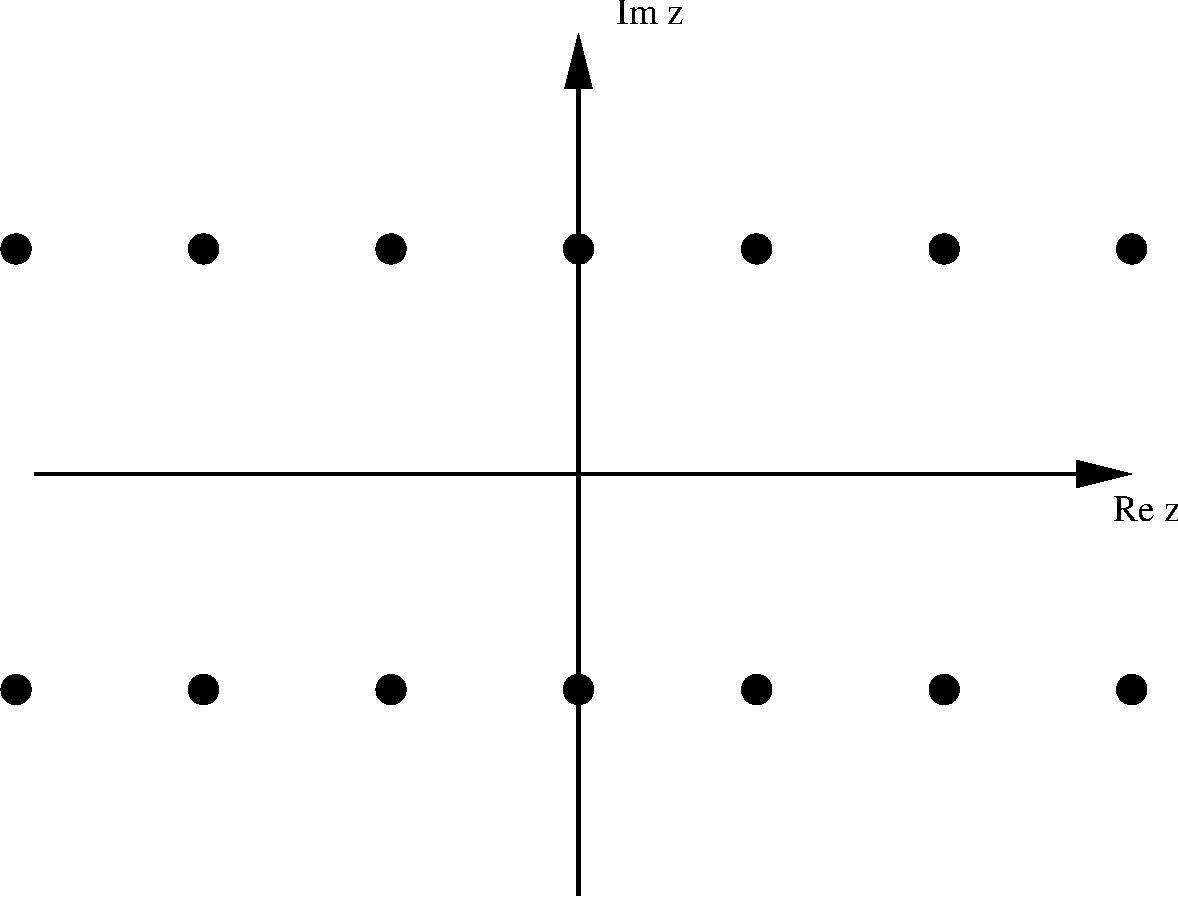
\includegraphics[width=.35\textwidth,angle=0]{A1.pdf}
\end{figure}

\sep
{\bf 3)} $f_0=0$, $ \ \ f_n = \frac{(-1)^{n+1}}{2^n}$ per $n \geq 1$; 
$ \ \ R=2$.

\sep
{\bf 4)} $x^2 \geq y^2$.
\begin{figure}[h]
\centering
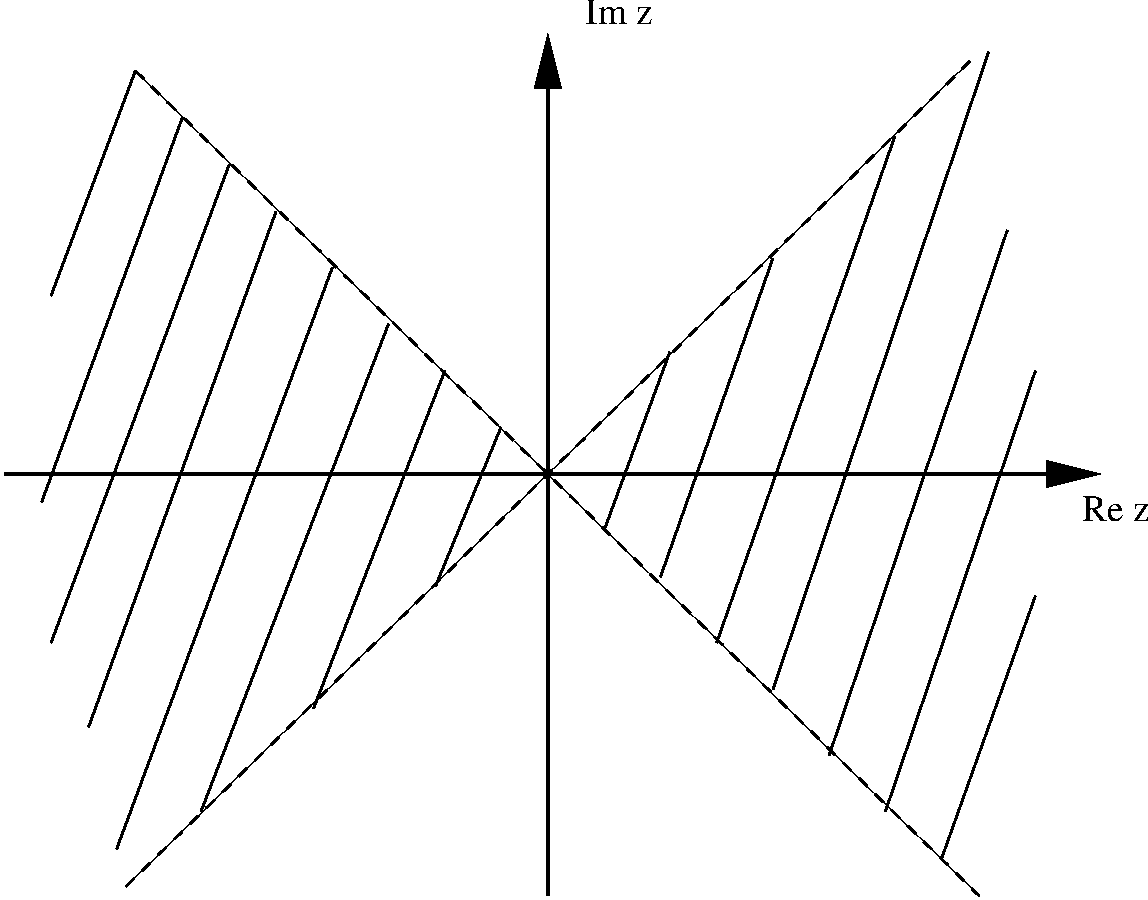
\includegraphics[width=.35\textwidth,angle=0]{A4.pdf}
\end{figure}

\sep
{\bf 5)} $z^3-8 i = (z-z_1)(z-z_2)(z-z_3)$;
$ \ \ z_1=\sqrt{3}+i$,$ \ \ z_2=-\sqrt{3}+i$,$ \ \ z_3=-2i$.

\newpage

\noindent
{\bf Compito B:}

\sep
{\bf 1)} $A(x,y)=(x^2+y^2) e^{x^2-y^2}$.

\sep
{\bf 2)} $z=z^\pm_n= \pm \log (2+\sqrt{3}) + 2\pi i n$, 
$ \ \ n=0,\pm 1,\pm 2, \dots$
\begin{figure}[h]
\centering
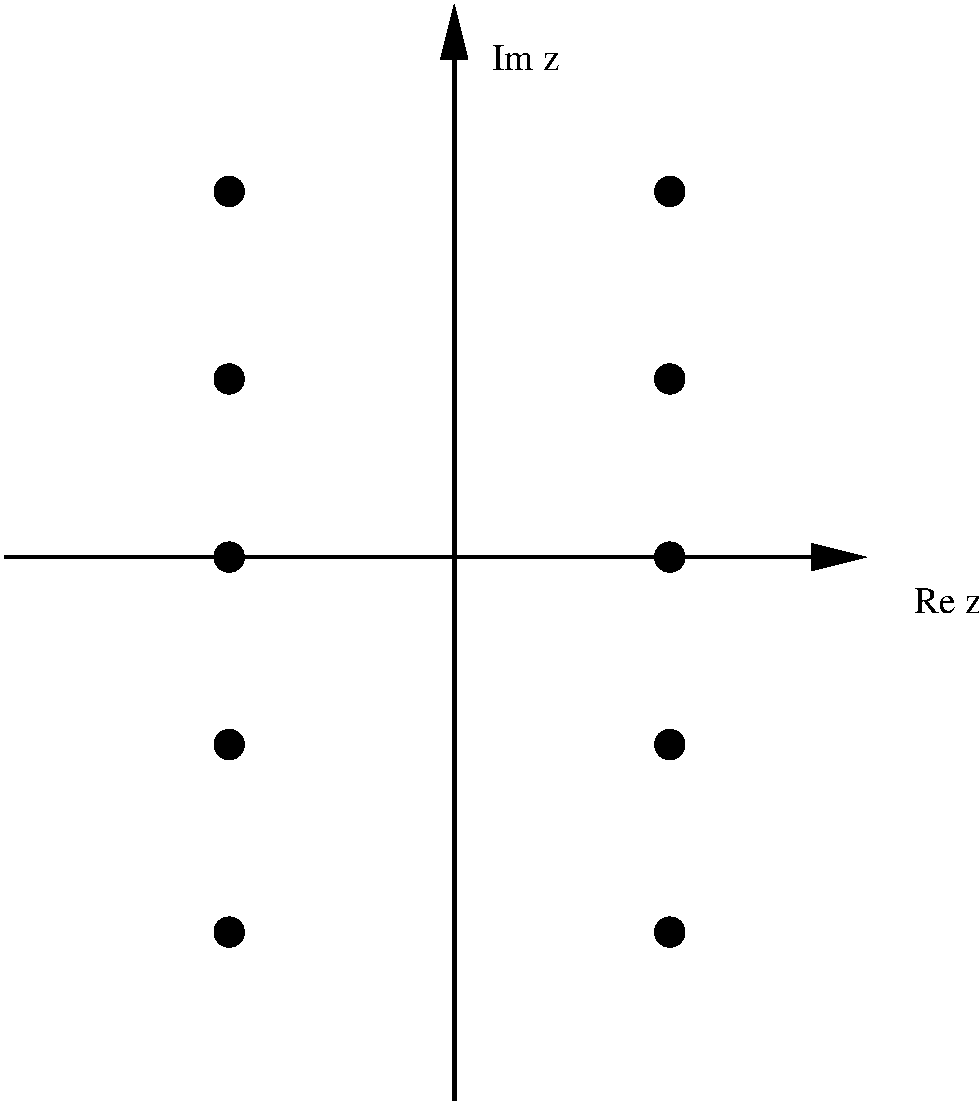
\includegraphics[width=.35\textwidth,angle=0]{B1.pdf}
\end{figure}

\sep
{\bf 3)} $f_0=f_1=0$, $ \ \ f_n = -\frac{1}{3^{n-1}}$ per $n \geq 2$; 
$ \ \ R=3$.

\sep
{\bf 4)} Im$(\sinh z) = \cosh x \sin y \geq 0 \ \ \Rightarrow \ \ \sin y \geq 0
\ \ \Rightarrow \ \ -\infty < x <\infty \ ,$ \\
$2\pi n \leq y \leq \pi + 2 \pi n \ , \ n=0,\pm 1,\pm 2, \dots$
\begin{figure}[h]
\centering
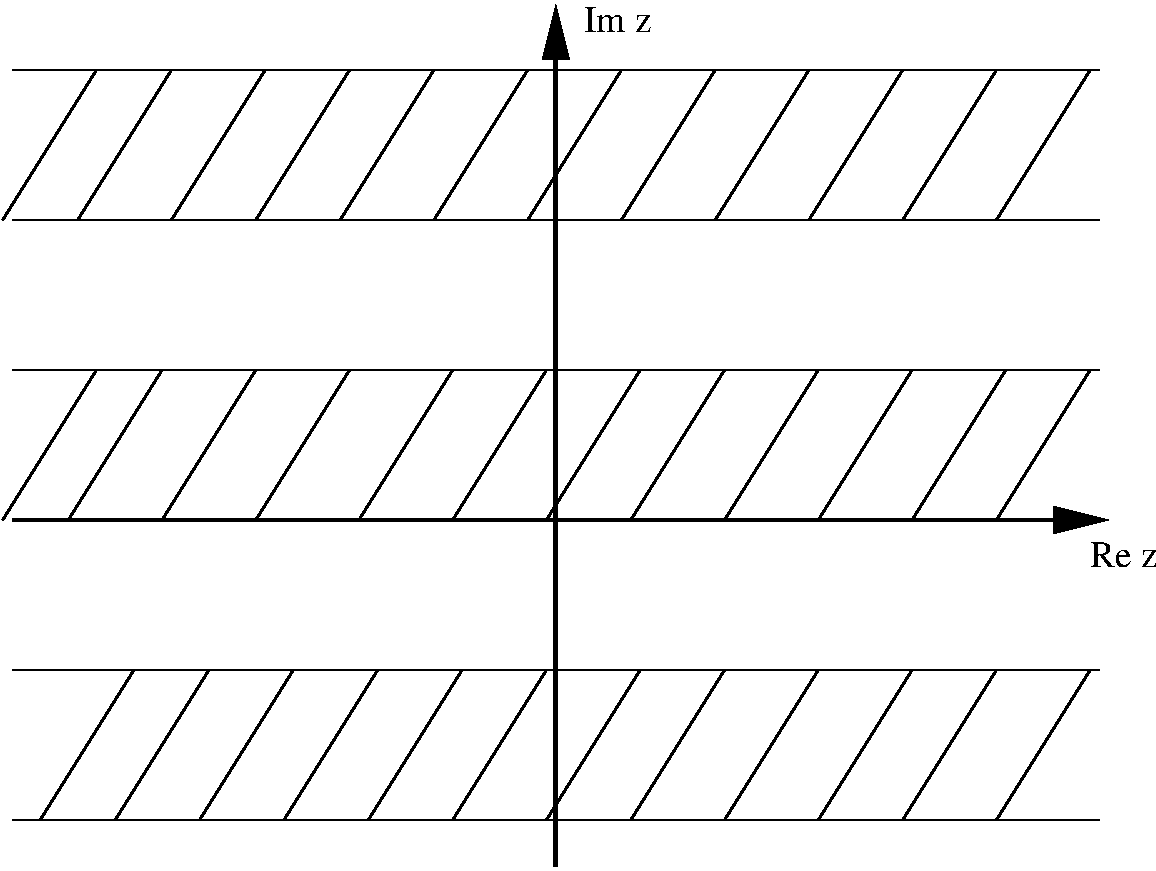
\includegraphics[width=.35\textwidth,angle=0]{B4.pdf}
\end{figure}

\sep
{\bf 5)} $z^4+16 = (z-z_1)(z-z_2)(z-z_3)(z-z_4)$;
$ \ \ z_1=\sqrt{2}(1+i)$,$ \ \ z_2=-\sqrt{2}(1+i)$,
$ \ \ z_3=\sqrt{2}(1-i)$,$ \ \ z_4=-\sqrt{2}(1-i)$.

\newpage

\noindent
{\bf Compito C:}

\sep
{\bf 1)} $A(x,y)=\frac{\sinh^2 x + \sin^2 y}{x^2 + y^2}$.

\sep
{\bf 2)} $z=z^\pm_n= \pm i \log (2+\sqrt{3}) + \frac{\pi}{2} + 2\pi n$, 
$ \ \ n=0,\pm 1,\pm 2, \dots$
\begin{figure}[h]
\centering
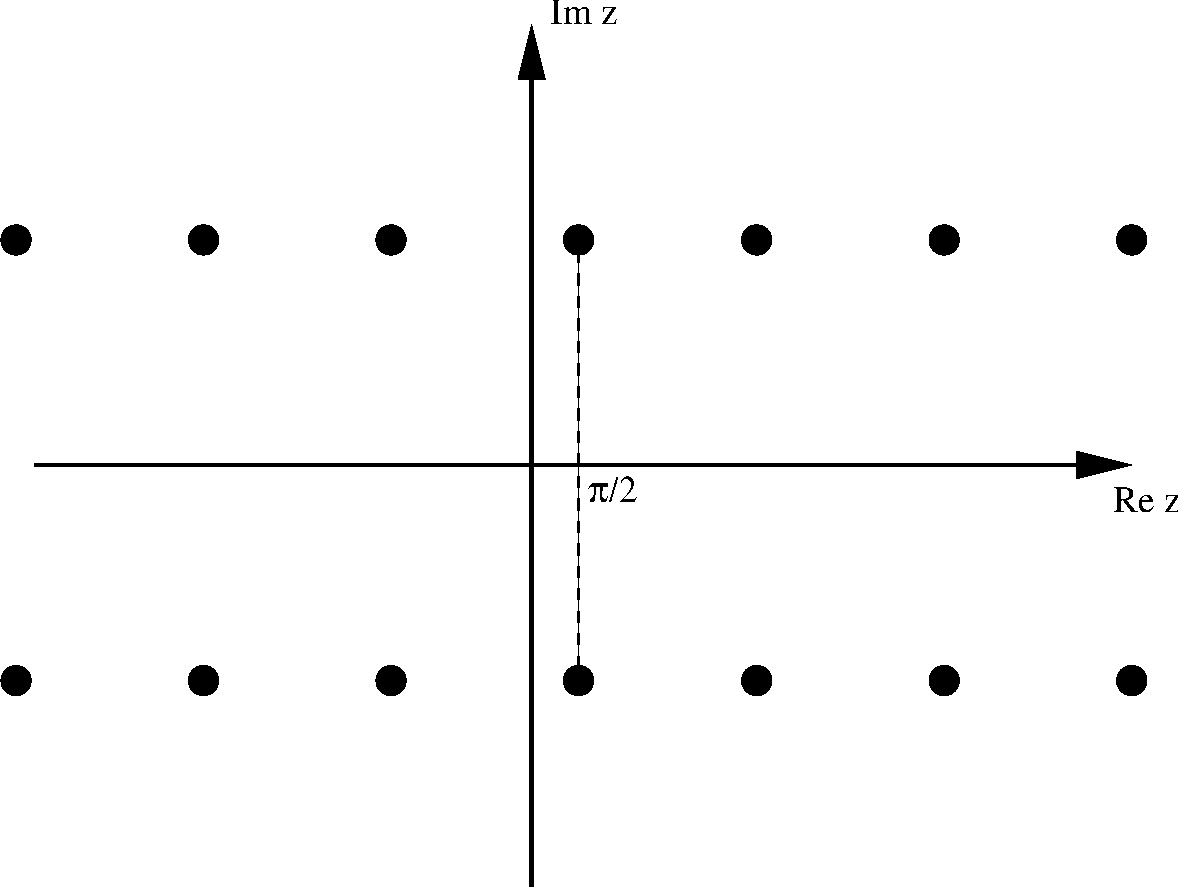
\includegraphics[width=.35\textwidth,angle=0]{C1.pdf}
\end{figure}

\sep
{\bf 3)} $f_n=0$ per $n=2p$, $ \ \ f_n = \frac{(-1)^{(n-1)/2}}{2^{(n+1)/2}}$
per $n = 2p+1$; $ \ \ R=\sqrt{2}$.

\sep
{\bf 4)} $\left( x + \frac{1}{2} \right)^2 \leq y^2$.
\begin{figure}[h]
\centering
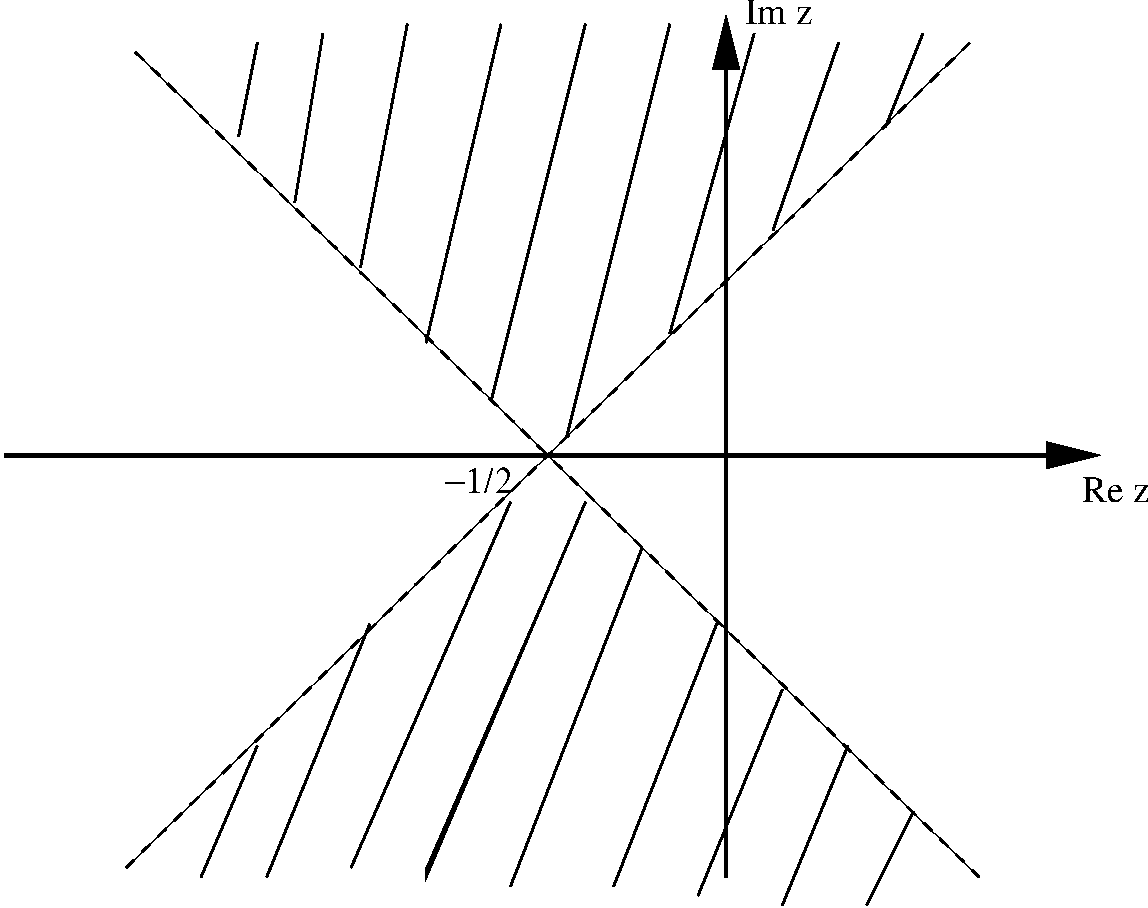
\includegraphics[width=.35\textwidth,angle=0]{C4.pdf}
\end{figure}

\sep
{\bf 5)} $z^3+27 = (z-z_1)(z-z_2)(z-z_3)$;
$ \ \ z_1=\frac{3}{2}+i \frac{3\sqrt{3}}{2}$,
$ \ \ z_2=\frac{3}{2}-i \frac{3\sqrt{3}}{2}$,$ \ \ z_3=-3$.

\newpage

\noindent
{\bf 6)} (comune ai tre compiti):

\sep
{\bf I)} Si scrive
\begin{equation}
P_n(z) = c_n z^n + c_{n-1} z^{n-1} + \cdots + c_1 z + c_0
\end{equation}
Se $P_n(z) = P_n(-z)$, allora $n$ \`e pari e $c_{n-1}=c_{n-3}=\cdots=c_1=0$
(tutti i coefficienti delle potenze dispari sono nulli). Scrivendo
\begin{equation}
P_n(z)=c_n (z-z_1)\cdots(z-z_n)
\end{equation}
si ha
\begin{equation}
c_{n-1}=-c_n \sum_{k=1}^n z_k = 0
\end{equation}
come volevasi dimostrare.

\sep
{\bf II)} Si osserva che se $z_1$ \`e soluzione di $P_n(z_1)=0$, 
anche $-z_1$ lo \`e. Allora
\begin{equation}
P_n(z)=(z-z_1)(z+z_1) P_{n-2}(z)=(z^2-z_1^2) P_{n-2}(z)
\end{equation}
e anche il polinomio $P_{n-2}(z)$ \`e pari essendo il rapporto di due funzioni
pari. Quindi se $z_2$ \`e soluzione di $P_{n-2}(z)=0$ (eventualmente 
coincidente con $z_1$) anche $-z_2$ \`e soluzione. E quindi
\begin{equation}
\begin{split}
& P_{n-2}(z) =(z-z_2)(z+z_2) P_{n-4}(z)=(z^2-z_2^2) P_{n-4}(z) \\
& P_n(z)=(z-z_1)(z+z_1)(z-z_2)(z+z_2) P_{n-4}(z)
\end{split}
\end{equation}
Iterando questa costruzione si vede che per ogni radice $z_p$ esiste la
corrispondente radice $-z_p$ e che la loro molteplicit\`a \`e la stessa,
e quindi
\begin{equation}
\sum_{k=1}^n z_k = \sum_{p=1}^{P} m_p z_p + \sum_{p=1}^{P} m_p (-z_p) = 0
\end{equation}
come volevasi dimostrare.

%%%%%%%%%%%%%%%%%%%%%%%%%%%%%%%%%%%%%%%%%%%%%%%%%%%%%%%%%%%%%%%%%%%%%%%%%%%%%%
%%%%%%%%%%%%%%%%%%%%%%%%%%%%%%%%%%%%%%%%%%%%%%%%%%%%%%%%%%%%%%%%%%%%%%%%%%%%%%

\newpage

\centerline{\bf ESERCITAZIONE III (10/02/2004)}

\sep

\noindent
{\bf Esercizio 1} - Calcolare tutti i possibili valori di $z=i^{\frac{1}{3}}$ 
e di $w=\log (\sqrt{2} + \sqrt{2} i)$.
\vskip.2cm \noindent
Risultato: $z_1 = \exp \frac{i \pi}{6}$, $z_2 = \exp \frac{5 i \pi}{6}$, $z_3 = \exp \frac{3 i \pi}{6} = -i$;
$w_n = \log 2 + i \left( \frac{\pi}{4} + 2n\pi\right), n=0, \pm 1, \pm 2, \ldots$.

\sep

\noindent
{\bf Esercizio 2} - Calcolare le soluzioni dell'equazione
\begin{equation} \nonumber
e^{\frac{1}{z}} = \alpha
\end{equation}
dove $\alpha$ \`e un numero complesso assegnato. Mostrare che se
$|\alpha|\neq 0$ il numero di soluzioni appartenenti al cerchio
$|z| \leq \varepsilon$ \`e infinito per qualunque $\varepsilon$.
\vskip.2cm \noindent
Risultato: $z_n = 1/(\log \alpha + 2\pi i n) \, , \, n=0, \pm 1, \pm 2, \ldots$

\sep

\noindent
{\bf Esercizio 3} - Dimostrare che la funzione
$f(z) = \overline{z} \tanh( \log z )^2$
non \`e analitica. 
\vskip.2cm \noindent
Suggerimento: usare la non-analiticit\`a della funzione $z\bar z=|z|^2$.

\sep

\noindent
{\bf Esercizio 4} - Sia $f(z) = u(x,y) + i v(x,y)$ analitica. Trovare la parte immaginaria $v(x,y)$ sapendo che: \\
a) $u(x,y) = x^3 + 3x(1-y^2)$ \ ; \\
b) $u(x,y) = \cos y \cosh x$ \ ; \\
c) $u(x,y) = e^{-x} [(1+x) \cos y + y \sin y]$ \ . 
\vskip.2cm \noindent
Risultato: a) $v(x,y) = -y^3 + 3y(1+x^2) + c$; b) $v(x,y)=\sinh x \sin y + c$; c) $v(x,y)=e^{-x} [-(1+x)
\sin y + y \cos y] + c$, dove $c$ \`e un numero reale arbitrario.

\sep

\noindent
{\bf Esercizio 5} - Scrivere esplicitamente $\int_\gamma f(z) dz$ in termini di una parametrizzazione della curva $\gamma$, se $\gamma$ \`e: \\
a) il triangolo di vertici $[0,1,i]$ percorso in senso orario; \\
b) la circonferenza di centro $i$ e raggio $R$ percorsa due volte in senso antiorario; \\
c) il quadrato di centro 0 e lato 2 percorso in senso antiorario.

\sep

\noindent
{\bf Esercizio 6} - Calcolare i seguenti integrali: \\
a) $I_a=\int_\gamma (z+1)^2 dz$ \ ; $\gamma$ \`e il triangolo di vertici $[-1,1,i]$ orientato in senso antiorario. \\
b) $I_b=\int_\gamma z \overline{z} \ dz$ \ ; $\gamma$ \`e la circonferenza di centro $z=0$ e raggio $R=5$ orientata in senso orario. \\
c) $I_c=\int_\gamma e^{\overline{z}} \ dz$ \ ; $\gamma$ \`e il quadrato di vertici $[0,1,1+i,i]$ orientato in senso antiorario. \\
d) $I_d=\int_\gamma \cosh{z} \ dz$ \ ; $\gamma$ \`e il quadrato di vertici $[0,1,1+i,i]$ orientato in senso antiorario.
\vskip.2cm \noindent
Risultato: $I_a = 0$; $I_b = 0$; $I_c = 2 (e-1) (1-e^{-i})$; $I_d=0$.

%%%%%%%%%%%%%%%%%%%%%%%%%%%%%%%%%%%%%%%%%%%%%%%%%%%%%%%%%%%%%%%%%%%%%%%%%%%%%%
%%%%%%%%%%%%%%%%%%%%%%%%%%%%%%%%%%%%%%%%%%%%%%%%%%%%%%%%%%%%%%%%%%%%%%%%%%%%%%

\newpage

\centerline{\bf ESERCITAZIONE IV (17/02/2004)}

\sep

\noindent
{\bf Esercizio 1} - Calcolare l'integrale $I_\gamma = \int_\gamma \bar{z} \ dz$ dove
$\gamma$ \`e una qualsiasi curva chiusa percorsa in senso antiorario.
\vskip.2cm \noindent
Risultato: usare il teorema di Gauss. $I_\gamma = 2i A_\gamma$, dove $A_\gamma$ \`e l'area
della porzione di piano interna a $\gamma$.

\sep

\noindent
{\bf Esercizio 2} - Sia $f(z) = u(x,y) + i v(x,y)$ analitica. Trovare $f(z)$ sapendo che $f(0)=0$ e che: \\
a) $u(x,y) = e^x [ (x^2- y^2) \cos y - 2 xy \sin y ] $ \ ; \\
b) $v(x,y) = 3 x^2 y  - y^3$ \ ; \\
c) $v(x,y) = \frac{y}{(x-1)^2 + y^2}$ \ . 
\vskip.2cm \noindent
Risultato: a) $f(z)=z^2 e^z$; b) $f(z)=z^3$; c) $f(z)=\frac{z}{1-z}$.

\sep

\noindent
{\bf Esercizio 3} - Calcolare i seguenti integrali: \\
a) $\int_\gamma \frac{e^{z-1}}{z-1} dz$ \ ; $\gamma$ \`e la circonferenza di centro $z=1$ e raggio $R=1$ orientata in senso antiorario. \\
b) $\int_\gamma  \frac{1}{|z|^2} \ dz$ \ ; $\gamma$ \`e la curva definita da $z(t) = \cosh t + i \sinh t$, $t \in (-\infty,\infty)$. Disegnare la curva $\gamma$. \\
c) $\int_\gamma \frac{1}{2z-i-1} \ dz$ \ ; $\gamma$ \`e il quadrato di vertici $[0,1,1+i,i]$ orientato in senso antiorario. \\
d) $\int_\gamma \frac{1}{z} \ dz$ \ ; $\gamma$ \`e l'ellisse di fuochi $z=1$ e $z=-1$ e asse principale $3$.\\
\vskip.2cm \noindent
Risultato: a) $2\pi i$; b) $i\pi/\sqrt{2}$; c) $\pi i$; d) $2\pi i$.


\sep

\noindent
{\bf Esercizio 4} - Calcolare il massimo del modulo della funzione $f(z)$ nel dominio ${\cal D}$, dove: \\
a) $f(z)=z^2$ \ ; ${\cal D}$ \`e il quadrato di vertici $[0,1,1+i,i]$. \\
b) $f(z)=\sinh^2 z$ \ ; ${\cal D}$ \`e il quadrato di vertici $[-1/2,1/2,1/2+2\pi i,-1/2+2\pi i]$. \\
c) $f(z)= z^2 + z$ \ ; ${\cal D}$ \`e il triangolo di vertici $[-1,1,i]$. \\
d) $f(z)=\frac{1}{z-3}$ \ ; ${\cal D}$ \`e il cerchio di centro $z=0$ e raggio $R=2$.
\vskip.2cm \noindent
Risultato: a) $2$; b) $\cosh^2 \frac{1}{2}$; c) $1$; d) $1$.

\sep

\noindent
{\bf Esercizio 5} - Sviluppare in serie di Laurent di centro $z_0$ le seguenti funzioni: \\
a) $f(z)=\frac{1}{(z-2)(z+3)}$ \ ; $z_0=2$. \\
b) $f(z)=\frac{1}{z^3-z^2-z+1}$ \ ; $z_0=1$. \\
c) $f(z)=\frac{e^z}{(z-z_0)^5}$ \ ; $\forall z_0$. \\
d) $f(z)=e^z + e^{\frac{1}{z}} - 1$ \ ; $z_0=0$.

%%%%%%%%%%%%%%%%%%%%%%%%%%%%%%%%%%%%%%%%%%%%%%%%%%%%%%%%%%%%%%%%%%%%%%%%%%%%%%
%%%%%%%%%%%%%%%%%%%%%%%%%%%%%%%%%%%%%%%%%%%%%%%%%%%%%%%%%%%%%%%%%%%%%%%%%%%%%%

\newpage

\centerline{\bf Esercizi di preparazione per il II esonero (27/02/2004)}

\sep
{\bf 1} - Scrivere i coefficienti $f_n$ della serie di Laurent:
\begin{equation} \nonumber
\begin{split}
&f(z)=\frac{z^2}{z-2} \sin \left( \frac{\pi z}{2z-4} \right) = \sum_{n=-\infty}^{\infty} f_n (z-2)^n \\
&f(z)=\frac{1}{z(z^2+4)}+\frac{z}{z^2+1}= \sum_{n=-\infty}^{\infty} f_n z^n \\
&f(z)=\frac{\sin \pi z}{(z-1)^2}+\frac{z}{z^2+2z-3}=\sum_{n=-\infty}^{\infty} f_n (z-1)^n \\
&f(z)=\frac{1}{z^2-iz+2}= \sum_{n=-\infty}^{\infty} f_n z^n
\end{split}
\end{equation}
in uno dei possibili domini di convergenza.

\sep
{\bf 2} - Determinare un polinomio armonico $P(x,y)$ tale che $P(1,0)=0$ e 
$P(0,1)=1$.

\sep
{\bf 3} - Sia $f(z)=u(x,y)+i v(x,y)$ analitica. Determinare $f(z)$ sapendo che: \\
a) $u(x,y)=3 x^2 (1-2y) + y^2 (2y-3)$ e $v(1,0)=2$. \\
b) $u(x,y)=(x^2-y^2) \cos x\cosh y + 2xy \sin x\sinh y$ e $f(0)=0$. \\
c) $v(x,y)=3x^3 + (1-y)(9xy-1)$ e $f(0)=0$. \\
Trovare i punti in cui $f(z)=0$.

\sep
{\bf 4} - Calcolare i seguenti integrali: \\
\begin{equation} \nonumber
\begin{split}
&I_1=\int_{0}^{2\pi} d\theta \ \frac{1+\cos^2\theta}{1+\sin^2\theta} \ ; \
I_2=\int_{0}^{2\pi} d\theta \ \frac{e^{-2i\theta}\sin\theta}{2+\sin\theta} \ ; \
I_3=\int_{-\infty}^{\infty} dx \ \frac{1+x^2}{(x^2 - 2x +2)(x^2 - 3ix - 2)} \ ; \\
&I_4=\int_{0}^{2\pi} d\theta \ \frac{1}{2+\cos\theta} \ ; \
I_5=\int_{0}^{\infty} dx \ \frac{\cos \pi x}{1+4 x^2} \ ; \
I_6=\int_{0}^{\infty} dx \ \frac{1 + \cos \pi x}{x^2+1} \ .
\end{split}
\end{equation}

\newpage

\sep
{\bf 5} - Calcolare i seguenti integrali (tutte le curve sono orientate in senso antiorario): \
\begin{equation} \nonumber
\begin{split}
& I_1=\int_\gamma dz \ z \overline{z} \ ; \ \ \text{$\gamma$ \`e il triangolo di vertici $[0,1,i]$.} \\
& I_2=\int_\gamma d\overline{z} \ (z-1)^2 \ ; \ \ \text{$\gamma$ \`e l'unione della semicirconferenza $|z-1|=1/2$, Im$z>0$} \\
& \hspace{5cm} \text{e del segmento di asse reale da essa sotteso.} \\
& I_3=\int_\gamma dz \ (z+\overline{z}) \ ; \ \ \text{$\gamma$ \`e il quadrato di vertici $[0,1,i+1,i]$.} \\
\end{split}
\end{equation}


\sep
{\bf 6} - Calcolare i seguenti integrali (tutte le curve sono orientate in senso antiorario): \\
\begin{equation} \nonumber
\begin{split}
& I_1=\int_\gamma dz \ \frac{\sin \pi z}{(z^2-4)(z-2)^2} \ ; \ \ \text{$\gamma$ \`e la circonferenza $|z-1-i|=2$.} \\
& I_2(n)=\frac{1}{2\pi i}\int_\gamma dz \ \frac{1 + z}{z^n (z^2+4)} \ ; \ \ \text{$\gamma$ \`e la circonferenza $|z|=1$, $n \in \mathbb{Z}$.} \\
& I_3=\int_\gamma dz \ \frac{z^4}{\sinh^2 z} \ ; \ \ \text{$\gamma$ \`e la circonferenza $|z-5i|=3$.} \\
& I_4=\int_\gamma dz \ \frac{z^3-6z}{(z^4+4)(z+2i)} \ ; \ \ \text{$\gamma$ \`e il quadrato con centro nell'origine, lati paralleli agli assi e lato 3.} \\
& I_5=\int_\gamma dz \ \frac{3z^4+5}{z^5+2} \ ; \ \ \text{$\gamma$ \`e la circonferenza $|z|=2$.} \\
& I_6=\int_\gamma dz \ \frac{z^3}{(z^2+1)^5} \ ; \ \ \text{$\gamma$ \`e la circonferenza $|z-1|=2$.} \\
\end{split}
\end{equation}

\sep
{\bf 7} - Calcolare i seguenti integrali per $k \in \mathbb{R}$: \\
\begin{equation} \nonumber
\begin{split}
&f_1(k)=\int_{-\infty}^\infty dx \ e^{ikx} \ \frac{x}{(x^2+1)^2} \ ; \
f_2(k)=\int_{-\infty}^\infty dx \ \ \frac{\cos kx}{x^2-2x+2} \ ; \
f_3(k)=\int_{0}^\infty dx \ \ \frac{\cos kx}{(x^2+1)} \ ; \\
&f_4(k)=\int_{0}^\infty dx \ \ \frac{x^2 \cos kx}{(x^2+1)^2} \ ; \
f_5(k)=\int_{-\infty}^\infty dx \ e^{-ikx} \ \frac{\sin x}{1+x^2} \ ; \
f_6(k)=\int_{-\infty}^\infty dx \ \ \frac{\cos 2kx}{x^4+5x^2+4} \ .
\end{split}
\end{equation}

%%%%%%%%%%%%%%%%%%%%%%%%%%%%%%%%%%%%%%%%%%%%%%%%%%%%%%%%%%%%%%%%%%%%%%%%%%%%%
%%%%%%%%%%%%%%%%%%%%%%%%%%%%%%%%%%%%%%%%%%%%%%%%%%%%%%%%%%%%%%%%%%%%%%%%%%%%%

\newpage

\centerline{\bf{METODI MATEMATICI DELLA FISICA}}

\centerline{\bf{II COMPITO D'ESONERO 2/03/04}}

\centerline{A.A. 2003-04 \ \ Prof.\ A.\ DEGASPERIS}

\centerline{\bf{COMPITO A}}
\vspace{20pt}
\noindent
{\bf ATTENZIONE}:

\noindent
scrivere su ciascun foglio il cognome ed indicare
\emph{chiaramente} l'inizio e la fine di ogni esercizio.
\vspace{20pt}
\noindent
\begin{enumerate}
\item Calcolare l'integrale $I=\oint_Cdz(1+2z^\ast)^2$ dove $C$ e' la
circonferenza $|z|=1$ orientata in senso antiorario 
..................[ 5 ] 
\item Sia $f(z)=u(x,y)+iv(x,y)$ una funzione intera
tale che $f(0)=0$, e sia $v(x,y)=4xy+3y+1-\exp(-y)
\cos(x)$ la sua parte immaginaria. Calcolare la sua
parte reale $u(x,y)$.................................[ 6 ]
\item Sia $C$ la
circonferenza $|z|=1$ orientata in senso antiorario, calcolare l'integrale
$A=\oint_Cdz\frac{z}{(z^2+4)(4z^2+1)}$
.........................[ 7 ]  
\item Calcolare il residuo in $z=i$ della funzione


$h(z)=\exp(4z)/(z^2+1)^2$..........................................
.........[ 6 ]
\item Calcolare l'integrale
$B=\int_{-\infty}^{+\infty}dxx^2/[(x+i)(x^2-2ix-2)^2]$..[ 6 ]
\item Dimostrare che, se $f(z)$ ha un polo od una singolarita'
\\essenziale in $z_0$, allora il residuo di $g(z)=df(z)/dz$ in $z_0$ e'
\\nullo........................................................
......................[ 7 ]
\end{enumerate}

\noindent IL NUMERO RIPORTATO ALLA FINE DI CIASCUN ESERCIZIO
E' IL VOTO MASSIMO. IL VOTO TOTALE E' LA SOMMA DEI 6 VOTI
PARZIALI (con riserva di una eventuale rinormalizzazione).

\newpage

\centerline{\bf{METODI MATEMATICI DELLA FISICA}}

\centerline{\bf{II COMPITO D'ESONERO 2/03/04}}

\centerline{A.A. 2003-04 \ \ Prof.\ A.\ DEGASPERIS}

\centerline{\bf{COMPITO B}}

\vspace{20pt}
\noindent
{\bf ATTENZIONE}:

\noindent
scrivere su ciascun foglio il cognome ed indicare
\emph{chiaramente} l'inizio e la fine di ogni esercizio.
\vspace{20pt}
\noindent
\begin{enumerate}
\item Calcolare l'integrale $I=\oint_Cdz(3z-{z^\ast}^2)^2$ dove $C$ e' la
circonferenza $|z|=1$ orientata in senso antiorario 
..................[ 5 ] 
\item Sia $f(z)=u(x,y)+iv(x,y)$ una funzione intera
tale che $f(0)=i$, e sia $u(x,y)=-4xy+x+\exp(x)
\sin(y)$ la sua parte reale. Calcolare la sua
parte immaginaria $v(x,y)$.....................................[ 6 ]
\item Sia $C$ la
circonferenza $|z-1|=1$ orientata in senso antiorario, calcolare
l'integrale
$A=\oint_Cdz\frac{1}{(4z^2-1)(4z^2-8z+5)}$
...................[ 7 ]  
\item Calcolare il residuo in $z=1$ della funzione
$h(z)=z\cos(\frac{\pi
z}{2})/(z-1)^3$.............[ 6 ]
\item Calcolare l'integrale
$B=\int_{0}^{2\pi}d\theta 1/[3-\cos(\theta )]$....................[ 6 ]
\item Dimostrare che, se $f(z)$ e' dispari, $f(-z)=-f(z)$, ed ha un polo
od una singolarita'
essenziale in $z=0$, allora il residuo di $g(z)=f(z)^2$ in $z=0$ e'
nullo...............[ 7 ]
\end{enumerate}
\vspace{20pt}

\noindent IL NUMERO RIPORTATO ALLA FINE DI CIASCUN ESERCIZIO
E' IL VOTO MASSIMO. IL VOTO TOTALE E' LA SOMMA DEI 6 VOTI
PARZIALI (con riserva di una eventuale rinormalizzazione).

\newpage

\centerline{\bf{METODI MATEMATICI DELLA FISICA}}

\centerline{\bf{II COMPITO D'ESONERO 2/03/04}}

\centerline{A.A. 2003-04 \ \ Prof.\ A.\ DEGASPERIS}

\centerline{\bf{COMPITO C}}
\vspace{20pt}
\noindent
{\bf ATTENZIONE}:

\noindent
scrivere su ciascun foglio il cognome ed indicare
\emph{chiaramente} l'inizio e la fine di ogni esercizio.
\vspace{20pt}
\noindent
\begin{enumerate}
\item Calcolare l'integrale $I=\oint_Cdz(z+z^\ast)^2/z^\ast$ dove $C$ e' la
circonferenza $|z|=1$ orientata in senso antiorario 
..................[ 5 ] 
\item Sia $f(z)=u(x,y)+iv(x,y)$ una funzione intera
tale che $f(0)=1$, e sia $u(x,y)=4x+x^2-y^2+\exp(2x)
\cos(2y)$ la sua parte reale. Calcolare la sua
parte immaginaria $v(x,y)$.........................[ 6 ]
\item Sia $C$ la
circonferenza $|z|=1$ orientata in senso antiorario, calcolare l'integrale
$A=\oint_Cdz\frac{z}{(z^2+3)(2z^2+3z-2)}$
.......................[ 7 ]  
\item Calcolare il residuo in $z=3$ della funzione \\
$h(z)=(z+1)\sin(\frac{\pi z}{2})/(z-3)^3$..............................
...............[ 6 ]
\item Calcolare l'integrale
$B=\int_{0}^{2\pi}d\theta \ 1/[9-8\sin^2 \theta]$.....................[ 6 ]
\item Dimostrare che, se $f(z)$ ha un polo od una singolarita'
\\essenziale in $z_0$, allora il residuo di $g(z)=df(z)/dz$ in $z_0$ e'
\\nullo........................................................
......................[ 7 ]
\end{enumerate}

\noindent IL NUMERO RIPORTATO ALLA FINE DI CIASCUN ESERCIZIO
E' IL VOTO MASSIMO. IL VOTO TOTALE E' LA SOMMA DEI 6 VOTI
PARZIALI (con riserva di una eventuale rinormalizzazione).

\newpage

\centerline {\bf SOLUZIONI II COMPITO D'ESONERO (02/03/2004)}

\sep
\noindent
{\bf Esercizio 1} \\ 
Si pone $z=e^{i\theta}$ da cui $z^*=e^{-i\theta}$ e
$dz=i e^{i\theta} d\theta$.
Sostituendo negli integrali e ricordando che
$\int_0^{2 \pi} d\theta \ e^{i m \theta} = 2\pi \delta_{m0}$
si ottiene: \\
A) $I=8 \pi i$ \tabb B) $I=-12\pi i$ \tabb C) $I=2 \pi i$ 

\sep
{\bf Esercizio 2} \\
A) $u(x,y)=2(x^2-y^2) + 3x + e^{-y} \sin x$, $\tabb f(z)= 2 z^2 + 3z +i -i e^{iz}$. \\
B) $v(x,y)=2(x^2-y^2) + y -e^x \cos y + 2$, $\tabb f(z)=2i z^2 + z -i e^z + 2i$. \\
C) $v(x,y)=4y + 2xy + e^{2x} \sin(2y)$, $\tabb f(z)=4z+z^2 + e^{2z}$.


\sep
{\bf Esercizio 3} \\
A) $A=2\pi i \left[ Res \left( \frac{z}{(z^2+4)(4z^2+1)} \right)_{\frac{i}{2}} +
Res \left( \frac{z}{(z^2+4)(4z^2+1)} \right)_{-\frac{i}{2}} \right] = \frac{2\pi i}{15}$. \\
B) $A=-2\pi i Res \left( \frac{1}{(4z^2-8z+5)(4z^2-1)} \right)_{-\frac{1}{2}} = \frac{\pi i}{20}$. \\
C) $A=2\pi i Res \left( \frac{z}{(2z^2+3z-2)(z^2+3)} \right)_{\frac{1}{2}} = \frac{4\pi i}{65}$.

\sep
{\bf Esercizio 4} \\
A) $Res[ h(z) ]_{i} = - \left( 1 + \frac{i}{4} \right) e^{4i}$. \\
B) $Res[ h(z) ]_{1} = -\frac{\pi}{2}$. \\
C) $Res[ h(z) ]_{3} = \frac{\pi^2}{2}$.

\sep
{\bf Esercizio 5} \\
A) Si chiude il cammino di integrazione su una semicirconferenza all'infinito nel semipiano inferiore (dove c'\`e un solo polo in $z=-i$) e quindi
$B = -2 \pi i Res \left( \frac{z^2}{(z+i)(z^2 - 2i z -2)^2} \right)_{-i} = \frac{2 \pi i}{25}$.
\sep
Per i compiti B e C si riscrive $\cos \theta = (z+z^{-1})/2$, $\sin \theta = (z-z^{-1})/2i$
e $d\theta = dz/iz$, dove $z$ varia sulla circonferenza goniometrica $C$ e quindi \\
B) $B=2 i \oint_C dz \frac{1}{z^2 - 6z + 1}=-4\pi Res \left( \frac{1}{z^2 - 6z +1} \right)_{3 - \sqrt{8}} = \frac{\pi}{\sqrt{2}}$. \\
C) $B=- i \oint_C dz \frac{z}{2z^4 +5z^2 + 2}=2 \pi \left[ Res \left( \frac{z}{2z^4 + 5z^2 +2} \right)_{\frac{i}{\sqrt{2}}} +  Res \left( \frac{z}{2z^4 + 5z^2 +2} \right)_{-\frac{i}{\sqrt{2}}} \right] = \frac{2\pi}{3}$

\newpage

\noindent
{\bf Esercizio 6} \\
Compiti A e C: \\
Per $0<|z-z_0|<R$, $f(z)=\cdots + \frac{f_{-n}}{(z-z_0)^n} + \cdots + 
\frac{f_{-1}}{(z-z_0)} + f_0 + f_1 (z-z_0) + \cdots$, quindi \\
$g(z)=\cdots - \frac{n f_{-n}}{(z-z_0)^{n+1}} + \cdots 
-\frac{f_{-1}}{(z-z_0)^2} + f_1 + 2 f_2 (z-z_0) + \cdots$ e questa serie di Laurent 
mostra che $Res[g(z)]_{z_0}=g_{-1}=0$.

\sep
Compito B: \\
Se $f(-z)=-f(z)$ allora $g(-z)=g(z)$ e quindi la serie di Laurent di $g(z)$ contiene solo
i termini pari:
$g(z)=\cdots + \frac{g_{-2n}}{z^{2n}} +  \frac{g_{-2n+2}}{z^{2n-2}} + \cdots 
+\frac{g_{-2}}{z^2} + g_0 + g_2 z^2 + \cdots + g_{2m} z^{2m} + \cdots$ e quindi
 $Res[g(z)]_{0}=g_{-1}=0$.

%%%%%%%%%%%%%%%%%%%%%%%%%%%%%%%%%%%%%%%%%%%%%%%%%%%%%%%%%%%%%%%%%%%%%%%%%%%%%%%
%%%%%%%%%%%%%%%%%%%%%%%%%%%%%%%%%%%%%%%%%%%%%%%%%%%%%%%%%%%%%%%%%%%%%%%%%%%%%%%

\newpage

\centerline{\bf ESERCITAZIONE V (9/3/2004)}

\sep
\noindent
{\bf 1} - Determinare un polinomio armonico $P(x,y)$ tale che: \\
a) $P(0,0)=0$, $P(0,1)=1$ e $P(1,1)=2$. \\
b) $P(0,-1)=1$, $P(-1,2)=2$. \\
c) $P(x,x)=x(3-2x^2)$. \\
d) $P(x,x^2)=x^4-x^2+1$. \\
e) $P(0,0)=3$, $\frac{\partial P}{\partial x}(1,0)=2$. \\
f) $P(1,1)=-1$, $\frac{\partial P}{\partial x}(0,0)=1$, 
$\frac{\partial P}{\partial y}(0,1)=0$.

\sep
{\bf 2} - Calcolare i seguenti integrali: \\
\begin{equation} \nonumber
\begin{split}
&I_1=\int_{0}^{\infty} dx \ \frac{\sqrt{x}}{x^2+5x+4} \ ; \
I_2=\int_{0}^{\infty} dx \ \frac{x^{2/3}}{x^2+4} \ ; \
I_3=\int_{0}^{\infty} dx \ \frac{1}{x^2+\sqrt{x}} \ ; \\
&I_4=\int_{-\infty}^{0} dx \ \frac{\sqrt[3]{x}}{(1-x)^2} \ ; \
I_5=\int_{-\infty}^{0} dx \ \frac{x^{-2/3}}{8-x} \ ; \
I_6=\int_{0}^{\infty} dx \ \frac{\sqrt[4]{x}}{x^2+5x+4} \ .
\end{split}
\end{equation}

\sep
{\bf 3} - Calcolare il residuo all'infinito delle seguenti funzioni: \\
\begin{equation} \nonumber
f(z)=\frac{z^2+1}{z^4-2} \ ; \ f(z)=e^{1/z} \ ; \ f(z)=e^{1/z^2} \ ; \ f(z)=\frac{z^5-2}{z^6+z^5+4} \ ; \ f(z)=\frac{z^4 + 4}{z^4 + 3 z^3} 
\end{equation}


\sep
{\bf 4} - Calcolare la trasformata di Fourier, $\hat{f}(k)=\int_{-\infty}^\infty dx \ e^{ikx} f(x)$, dove $f(x)$ \`e data da: \\
\begin{equation} \nonumber
\begin{split}
&f(x)=\exp \Big(-3x^2 \Big) \ ; \ f(x)=\exp \left[ -\frac{(x-1)^2}{3} \right] \ ; \ f(x)=e^{-x^2} \sin 4x \ ; \\
&f(x)=\frac{\sin 4x}{x^2+1} \ ; \ f(x)=\exp \Big( -|x| \Big) \ ; \
f(x)=\exp \Big( -|x+5| \Big)
\end{split}
\end{equation}
Se possibile, verificare che $f(x)=\int_{-\infty}^\infty \frac{dk}{2\pi} \ e^{-ikx} \hat{f}(k)$. \\
{\it Suggerimento:} Ricordate che potete ``completare il quadrato'', nel senso
che
\begin{equation} \nonumber
\int_{-\infty}^\infty dx \ e^{-A x^2 + B x} = \int_{-\infty}^\infty dx \ e^{-A (x-\frac{B}{2A})^2} \ e^{\frac{B^2}{4A}}
\end{equation}
A questo punto, se $A$ \`e reale e positivo, mostrate che, $\forall \alpha \in \mathbb{C}$,
\begin{equation} \nonumber
\int_{-\infty}^\infty dx \ e^{-A (x+\alpha)^2} = \sqrt{\frac{\pi}{A}} \ .
\end{equation}

%%%%%%%%%%%%%%%%%%%%%%%%%%%%%%%%%%%%%%%%%%%%%%%%%%%%%%%%%%%%%%%%%%%%%%%%%%%%%
%%%%%%%%%%%%%%%%%%%%%%%%%%%%%%%%%%%%%%%%%%%%%%%%%%%%%%%%%%%%%%%%%%%%%%%%%%%%%

\newpage

\begin{figure}
\centering
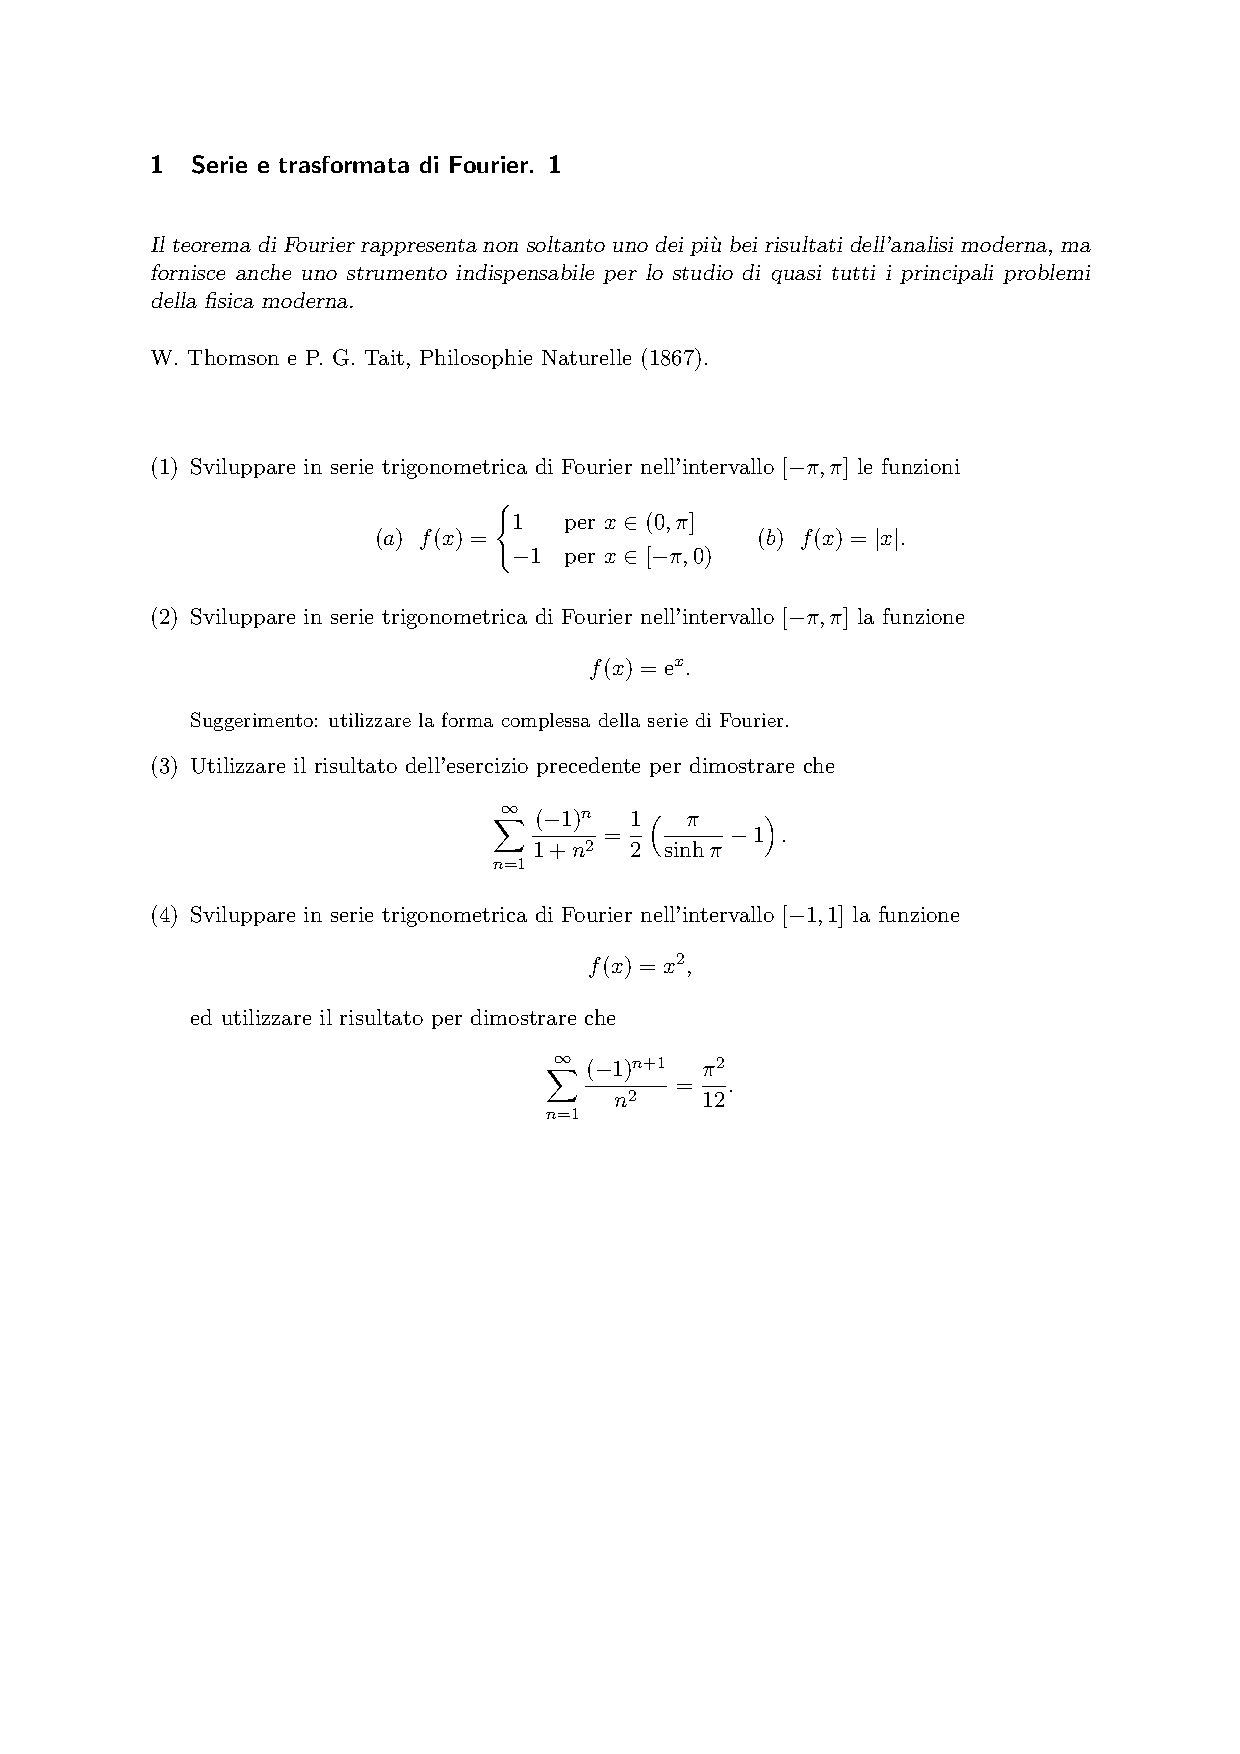
\includegraphics[width=1.2\textwidth,angle=0]{fourier-1.pdf}
\end{figure}


\newpage

\centerline{\bf Simulazione del III esonero (16/03/2004)}

\sep
\noindent
{\bf 1} - Calcolare l'integrale
\begin{equation} \nonumber
I= \int_{-\infty}^0 dx \ \frac{x^{4/5}}{x^2-3x+2}
\end{equation}

\sep
{\bf 2} - Calcolare l'integrale
\begin{equation} \nonumber
\hat{f}(k)=\int_{-\infty}^{\infty} dx \ e^{i k x} \ \frac{x^2 \cos 6 x}{x^4+16}
\end{equation}

\sep
{\bf 3} - Calcolare l'integrale
\begin{equation} \nonumber
\hat{f}(k)=\int_{-\infty}^{\infty} dx \ e^{ikx} \ e^{-3 (x-1)^2} \sin 2 (x-1)
\end{equation}

\sep
{\bf 4} - Trovare una soluzione $f(x,y)$ dell'equazione di Laplace tale che,
sulla circonferenza di centro $(1,1)$ e raggio $1/2$, si abbia 
$f=8 x^3 - 12 x^2 - 6x + 4$.

\sep
{\bf 5} - Calcolare il residuo all'infinito di 
$f(z)=\frac{z^4}{z^3+9 z} + \cos \frac{1}{z^3}$.

\sep
{\bf 6} - Sviluppare in serie di Fourier la funzione 
$f(\theta)=\frac{1}{3 + \cos^2 \theta}$ nell'intervallo $-\pi \leq \theta \leq \pi$.

\sep
{\bf 7} - Sviluppare in serie di Fourier nell'intervallo $-\pi \leq \theta \leq \pi$ la funzione
\begin{equation} \nonumber
f(\theta)=\begin{cases} & \frac{\theta}{\pi}+1 \hspace{1cm} \theta \in [-\pi,0) \\
& 1 \hspace{1,5cm} \theta \in [0,\pi) 
\end{cases}
\end{equation}

%%%%%%%%%%%%%%%%%%%%%%%%%%%%%%%%%%%%%%%%%%%%%%%%%%%%%%%%%%%%%%%%%%%%%%%%%%%%%
%%%%%%%%%%%%%%%%%%%%%%%%%%%%%%%%%%%%%%%%%%%%%%%%%%%%%%%%%%%%%%%%%%%%%%%%%%%%%

\newpage

\centerline{\bf{METODI MATEMATICI DELLA FISICA}}

\centerline{\bf{III COMPITO D'ESONERO 22/03/04}}

\centerline{A.A. 2003-04 \ \ Prof.\ A.\ DEGASPERIS}
\centerline{\bf{COMPITO  A}}
\vspace{20pt}
\noindent
{\bf ATTENZIONE}:

\noindent
scrivere su ciascun foglio il cognome ed indicare
\emph{chiaramente} l'inizio e la fine di ogni esercizio.
\vspace{20pt}
\noindent
\begin{enumerate}
\item Calcolare l'integrale $I=\int_0^{+\infty}dx\frac{x}{x^3+1}$
..................................[ 6 ] 
\item Calcolare, per ogni $k$ reale, l'integrale di Fourier
 
$F(k)=\int_{-\infty}^{+\infty}dx\frac{x\exp(ikx)}{(x^2+1)^2}$
........................................................[ 6 ]
\item Calcolare il residuo in $z_0=\infty$ della funzione

$f(z)=\frac{z^2}{1+4z^2} \sin(2/z)$ ..........................
...............................[ 5 ]  
\item Calcolare la serie di Fourier 
$g(x)=\sum_{n=1}^{\infty} \frac{(-1)^n}{2^n}\sin(2nx)$
nell'intervallo $-\pi<x<\pi$.............................
.........................................[ 6 ]
\item Sia, nell'intervallo $-\pi<x<\pi$, $1/[4+\cos(x)
]=\sum_{n=-\infty}^{+\infty} c_n \exp(inx)$. Calcolare i coefficienti di
Fourier $c_n$ per ogni intero $n$.....[ 6 ]
\item Se la funzione $A(z)$ e' analitica in $z=0$ ed e' dispari,
$A(-z)=-A(z)$, mostrare che la funzione $B(z)=\sqrt zA(\sqrt z)$ e'
analitica in
$z=0$........................................................
.......................[ 6 ]

\end{enumerate}

\noindent IL NUMERO RIPORTATO ALLA FINE DI CIASCUN ESERCIZIO
E' IL VOTO MASSIMO. IL VOTO TOTALE E' LA SOMMA DEI 6 VOTI
PARZIALI (con riserva di una eventuale rinormalizzazione).

\newpage

\centerline{\bf{METODI MATEMATICI DELLA FISICA}}

\centerline{\bf{III COMPITO D'ESONERO 22/03/04}}

\centerline{A.A. 2003-04 \ \ Prof.\ A.\ DEGASPERIS}
\centerline{\bf{COMPITO  B}}
\vspace{20pt}
\noindent
{\bf ATTENZIONE}:

\noindent
scrivere su ciascun foglio il cognome ed indicare
\emph{chiaramente} l'inizio e la fine di ogni esercizio.
\vspace{20pt}
\noindent
\begin{enumerate}
\item Calcolare l'integrale $I=\int_0^{+\infty}dx\frac{x^{1/2}}{x^3+1}$
..................................[ 6 ] 
\item Calcolare, per ogni $k$ reale, l'integrale di Fourier
 
$F(k)=\int_{-\infty}^{+\infty}dx\frac{x^2\exp(ikx)}{(4x^2+1)^2}$
........................................................[ 6 ]
\item Calcolare il residuo in $z_0=\infty$ della funzione

$f(z)=(\frac{4}{z}+z) \cosh(2z^2)$ ......................
...............................[ 5 ]  
\item Calcolare la serie di Fourier 
$g(x)=\sum_{n=-\infty}^{+\infty} \frac{1}{3^{|n|}}\exp(inx)$
nell'intervallo $-\pi<x<\pi$.............................
.........................................[ 6 ]
\item Sia, nell'intervallo $-\pi<x<\pi$, $1/[3-\sin(x)
]=\sum_{n=-\infty}^{+\infty} c_n \exp(inx)$. Calcolare i coefficienti di
Fourier $c_n$ per ogni intero $n$.....[ 6 ]
\item Sia $P(z)$ un polinomio della variabile
$z=x+iy$  e siano i polinomi $a(x,y)=Re[P(z)]$ e
$b(x,y)=Im[P(z)]$. Mostrare che il polinomio
$q(x,y)=a(x,y) b(x,y)$ e' armonico......................[ 6 ]

\end{enumerate}

\noindent IL NUMERO RIPORTATO ALLA FINE DI CIASCUN ESERCIZIO
E' IL VOTO MASSIMO. IL VOTO TOTALE E' LA SOMMA DEI 6 VOTI
PARZIALI (con riserva di una eventuale rinormalizzazione).

\newpage

\centerline{\bf{METODI MATEMATICI DELLA FISICA}}

\centerline{\bf{III COMPITO D'ESONERO 22/03/04}}

\centerline{A.A. 2003-04 \ \ Prof.\ A.\ DEGASPERIS}
\centerline{\bf{COMPITO  C}}
\vspace{20pt}
\noindent
{\bf ATTENZIONE}:

\noindent
scrivere su ciascun foglio il cognome ed indicare
\emph{chiaramente} l'inizio e la fine di ogni esercizio.
\vspace{20pt}
\noindent
\begin{enumerate}
\item Calcolare l'integrale $I=\int_0^{+\infty}dx\frac{x^{1/3}}{x^3+1}$
..................................[ 6 ] 
\item Calcolare, per ogni $k$ reale, l'integrale di Fourier
 
$F(k)=\int_{-\infty}^{+\infty}dx\frac{\exp(ikx)}{(x^2+4)^2}$
..........................................................[ 6 ]
\item Calcolare il residuo in $z_0=\infty$ della funzione

$f(z)=(1+z)^4 \sin ^2(1/z^2)$ ..........................
.........................[ 5 ]  
\item Calcolare la serie di Fourier 
$g(x)=\sum_{n=0}^{\infty} \frac{1}{n!}\cos(nx)$
nell'intervallo $-\pi<x<\pi$.....[ 6 ]
\item Sia, nell'intervallo $-\pi<x<\pi$, $\sin(x)/[2+\cos(x)
]=\sum_{n=-\infty}^{+\infty} c_n \exp(inx)$. Calcolare i coefficienti di
Fourier $c_n$ per ogni intero $n$.....[ 6 ]
\item Mostrare che la serie di Fourier
$A(x)=\sum_{n=0}^{=\infty}(1/3^n)\cos(nx)$ converge
uniformemente nell'intervallo $-\pi<x<\pi$
............[ 6 ]

\end{enumerate}

\noindent IL NUMERO RIPORTATO ALLA FINE DI CIASCUN ESERCIZIO
E' IL VOTO MASSIMO. IL VOTO TOTALE E' LA SOMMA DEI 6 VOTI
PARZIALI (con riserva di una eventuale rinormalizzazione).

\newpage


\centerline{\bf SOLUZIONI III COMPITO D'ESONERO (22/03/2004)}
\sep
\noindent
{\bf Esercizio 1} \\
\begin{equation} \nonumber
\begin{split}
& A) \tabb I=\int_0^\infty dx \ \frac{x}{x^3+1}=
-\sum \text{Res} \left( \frac{z \log z}{1+z^3} \right)
=-\sum_k \frac{\log z_k}{3 z_k} = \frac{2 \pi}{3 \sqrt{3}} \\
& B) \tabb I=\int_0^\infty dx \ \frac{x^{1/2}}{1+x^3}=
\pi i \sum \text{Res} \left( \frac{z^{1/2}}{1+z^3} \right) 
=\pi i \sum_k \frac{z_k^{1/2}}{3 z_k^2} = \frac{\pi}{3} \\
 & C) \tabb I=\int_0^\infty dx \ \frac{x^{1/3}}{1+x^3}=
\frac{ 2\pi i}{1-e^{2\pi i/3}} 
\sum \text{Res} \left( \frac{z^{1/3}}{1+z^3} \right) 
=\frac{\pi e^{2\pi i/3}}{\sin (\pi/3)}
\sum_k \frac{z_k^{1/3}}{3 z_k^2} =
\frac{2\pi}{3 \sqrt{3}} \left(2 \cos \frac{\pi}{9} - 1\right)
\end{split}
\end{equation}
dove $z_k=\Big\{e^{i\pi/3},e^{i\pi},e^{5i\pi/3}\Big\}$ e la penultima
uguaglianza \`e ottenuta usando la formula di De L'Hopital,
\begin{equation} \nonumber
\lim_{z \rightarrow z_i} \frac{z-z_i}{1+z^3} = \frac{1}{3 z_i^2}
\end{equation}

\sep
{\bf Esercizio 2} \\
Si deve calcolare un integrale tipo $F(k)=\int_{-\infty}^\infty dx e^{ikx} f(x)$. \\
A) Per $k > 0$ si chiude il cammino di integrazione nel semipiano superiore e
\begin{equation} \nonumber
F_+(k)=2\pi i \Res \left[ e^{i k z} \frac{z}{(z^2+1)^2} \right]_{z=i}=
2 \pi i \lim_{z\rightarrow i} \frac{d}{dz} e^{i k z} \frac{z (z-i)^2}{(z^2+1)^2} =
\frac{\pi}{2} i k e^{-k}
\end{equation}
Dal momento che la funzione $f(x)$ \`e dispari, si ha $F(k)=-F(-k)$ e quindi per 
$k<0$ si ha
\begin{equation} \nonumber
F_-(k)=-F_+(-k)=\frac{\pi}{2} i k e^{k}
\end{equation}
e infine, $\forall k \in \mathbb{R}$, $F(k)=\frac{\pi}{2} i k e^{-|k|}$. 
Alternativamente, si pu\`o calcolare $F_-(k)$ chiudendo il cammino nel semipiano
inferiore. \\
B) Come nel caso precedente per $k>0$
\begin{equation} \nonumber
F_+(k)=2\pi i \Res \left[ e^{i k z} \frac{z^2}{(4z^2+1)^2} \right]_{z=i/2}=
2 \pi i \lim_{z\rightarrow i/2} \frac{d}{dz} e^{i k z} \frac{z^2 (z-i/2)^2}{(4z^2+1)^2} =
\frac{\pi}{32} (2-k) e^{-k/2}
\end{equation}
Stavolta la funzione $f(x)$ \`e pari, quindi $F(k)=F(-k)$ e per $k<0$ si ha
\begin{equation} \nonumber
F_-(k)=F_+(-k)=\frac{\pi}{32} (2+k) e^{k/2}
\end{equation}
e infine, $\forall k \in \mathbb{R}$, $F(k)=\frac{\pi}{32} (2-|k|) e^{-|k|/2}$. \\
C) Come nel caso precedente per $k>0$
\begin{equation} \nonumber
F_+(k)=2\pi i \Res \left[ e^{i k z} \frac{1}{(z^2+4)^2} \right]_{z=2i}=
2 \pi i \lim_{z\rightarrow 2i} \frac{d}{dz} e^{i k z} 
\frac{(z-2i)^2}{(z^2+4)^2} =
\frac{\pi}{16} (1+2k) e^{-2k}
\end{equation}
e $F(k)=F(-k)$ per cui $F(k)=\frac{\pi}{16} (1+2|k|) e^{-2|k|}$.

\sep
{\bf Esercizio 3} \\
\begin{equation} \nonumber
\begin{split}
&A) \tabb f\left(\frac{1}{w}\right)=\frac{1}{4+w^2} \sin 2w =
\left[ \frac{1}{4}-\frac{w^2}{16}+o(w^4)\right][2w+o(w^3)] = \frac{w}{2} + o(w^2)  \tabb \Res f_\infty = -\frac{1}{2} \\
&B) \tabb f(z)=\left(\frac{4}{z}+z \right) \left[1+2 z^4 + \frac{2}{3} z^8 + \cdots\right] = 
\frac{4}{z} + z + 8 z^3 + 2 z^5 + \cdots \tabb \tabb \Res f_\infty = -4 \\
&C) \tabb f(z)=(z^4+4z^3+6z^2+4z+1)
\left( \frac{1}{z^4}-\frac{1}{3z^8} + \cdots \right) = 1 + \frac{4}{z} + \cdots
\tabb \tabb \Res f_\infty = -4
\end{split}
\end{equation}

\sep
{\bf Esercizio 4} \\
\begin{equation} \nonumber
\begin{split}
&A) \tabb g(x)= \text{Im} \sum_{n=1}^\infty \left( -\frac{1}{2} \right)^n e^{2nxi} =
\text{Im} \left[ \frac{1}{1+\frac{1}{2}e^{2xi}} - 1 \right] = 
-\frac{2\sin 2x}{5 + 4 \cos 2x} \\
&B) \tabb g(x)= 1 + \sum_{n=1}^\infty \frac{e^{inx}}{3^n} + 
\sum_{n=1}^\infty \frac{e^{-inx}}{3^n} = 
1 + 2 \text{Re} \sum_{n=1}^\infty \frac{e^{inx}}{3^n} =
1 +  2 \text{Re} \left[ \frac{1}{1-e^{ix}/3} - 1 \right] = 
\frac{4}{5 -3 \cos x} \\
&C) \tabb g(x) = \text{Re} \sum_{n=0}^\infty \frac{(e^{ix})^n}{n!} =
\text{Re} \ e^{e^{ix}} = e^{\cos x} \cos \sin x
\end{split}
\end{equation}

\sep
{\bf Esercizio 5} \\
A) Dalle formule per i coefficienti di Fourier si ha
\begin{equation} \nonumber
c_n = \frac{1}{2\pi} \int_{-\pi}^\pi dx \frac{e^{-inx}}{4+\cos x} =
\frac{1}{\pi i} \oint dz \frac{z^{-n}}{z^2 + 8 z + 1}
\end{equation}
dove l'integrale \`e fatto sulla circonferenza di raggio 1.
Per $n\geq 0$ la funzione va a zero pi\`u velocemente di $1/z^2$ all'infinito
quindi conviene sommare i residui esterni alla circonferenza.
L'unico polo esterno \`e in $z=-4-\sqrt{15}$ e
\begin{equation} \nonumber
c_n=-2 \Res \left[ \frac{z^{-n}}{z^2 + 8 z + 1} \right]_{-4-\sqrt{15}} = 
\frac{(-1)^n}{(4+\sqrt{15})^n \sqrt{15}}
\end{equation}
Dal momento che la funzione \`e pari si ha $c_{-n}=c_n$ e quindi per $n<0$
\begin{equation} \nonumber
c_{n}=\frac{(-1)^n}{(4+\sqrt{15})^{-n} \sqrt{15}}=
\frac{(-1)^n}{(4-\sqrt{15})^n \sqrt{15}}
\end{equation}
B) Come nel caso precedente
\begin{equation} \nonumber
c_n = \frac{1}{2\pi} \int_{-\pi}^\pi dx \frac{e^{-inx}}{3-\sin x} =
\frac{1}{\pi} \oint dz \frac{z^{-n}}{-z^2 + 6 i z + 1}
\end{equation}
In questo caso la funzione non ha parit\`a definita per cui bisogna 
considerare separatamente $n>0$ e $n\leq 0$.
Consideriamo prima il caso $n\leq 0$: la funzione ha un solo polo interno alla
circonferenza di raggio 1 in $z=(3-2\sqrt{2})i$ e
\begin{equation} \nonumber
c_n= 2i \Res \left[ \frac{z^{-n}}{-z^2 + 6 i z + 1} \right]_{(3-2\sqrt{2})i} = 
\frac{1}{i^n (3-2\sqrt{2})^n 2\sqrt{2}}
\end{equation}
Per $n>0$ invece come nel caso precedente si considera il residuo esterno
in $z=(3+2\sqrt{2})i$ e
\begin{equation} \nonumber
c_n= -2i \Res \left[ \frac{z^{-n}}{-z^2 + 6 i z + 1} \right]_{(3+2\sqrt{2})i} = 
\frac{1}{i^n (3+2\sqrt{2})^n 2\sqrt{2}}
\end{equation}
C) Come nel caso precedente
\begin{equation} \nonumber
c_n = \frac{1}{2\pi} \int_{-\pi}^\pi dx \frac{\sin x \ e^{-inx}}{2+\sin x} =
-\frac{1}{2\pi} \oint dz \frac{(z^2+1) \ z^{-n-1}}{(z-z_+)(z-z_-)}
\end{equation}
con $z_\pm=-2 \pm \sqrt{3}$. Si ottiene come nel caso precedente
\begin{equation} \nonumber
c_n=
\begin{cases}
&i z_+^n \tabb n \geq 1 \\
&0 \tabb n = 0 \\
&-i z_+^{-n} \tabb n \leq 1 
\end{cases}
\end{equation}
ovvero $c_n=i \ \text{sgn} n \ (\sqrt{3}-2)^{|n|}$.

\sep
{\bf Esercizio 6} \\
A) $A(z)=\sum_{n=0}^\infty a_n z^{2n+1} \Rightarrow
A(\sqrt{z})=\sum_{n=0}^\infty a_n z^{n+1/2} \Rightarrow
B(z)=\sqrt{z} A(\sqrt{z})=\sum_{n=0}^\infty a_n z^{n+1}$, e quindi \`e analitica
in $z=0$ per definizione. \\
B) $P(z)=a + i b \Rightarrow P^2(z)=a^2-b^2 +2i ab \Rightarrow a b = \text{Im} P^2(z)/2$
e quindi \`e un polinomio armonico. \\
C) $|\sum_{n=0}^\infty (1/3^n) \cos (nx)| \leq \sum_{n=0}^\infty |(1/3^n) \cos (nx)|
\leq \sum_{n=0}^\infty (1/3^n) = 3/2$. Il termine n-esimo della serie \`e stimato
uniformemente dal termine n-esimo di una serie convergente, quindi la serie converge
uniformemente. \\
{\it oppure} si somma la serie $A(x)=\text{Re} 
\sum_{n=0}^\infty \left( \frac{e^{ix}}{3} \right)^n = \frac{3 (3-\cos x)}{10-6 \cos x}$
e poich\'e $A(x)$ \`e continua in $-\pi \leq x \leq \pi$ e periodica, $A(x+2\pi)=A(x)$,
per il teorema di Fejer la serie di Fourier converge uniformemente.

\newpage

\centerline{\bf METODI MATEMATICI DELLA FISICA}

\centerline{\bf COMPITO D'ESAME 29/03/04}

\centerline{A.A. 2003-04 \ \ Prof.\ A.\ DEGASPERIS}
\vspace{20pt}
\noindent
{\bf ATTENZIONE}:

\noindent
scrivere su ciascun foglio il cognome ed indicare
\emph{chiaramente} l'inizio e la fine di ogni esercizio.
\vspace{20pt}
\noindent
\begin{enumerate}
\item Sia $f(z)=\sum_{n=0}^{+\infty}f_n (z-1)^n$ lo sviluppo in serie di
Taylor della funzione $f(z)=(2z^2-z-1)/(4z^2-4z-3)$ in $z_0=1$.
Calcolare i coefficienti $f_n$ ed il raggio di convergenza $R$. 
..................[ 5 ] 
\item Trovare le 4 radici del polinomio
$P(z)=9z^4+4$................[ 5 ]
\item Sia $g(z)=(z^2-4)/[(z^2+1)(z^2+7z+10)]$, calcolare l'integrale
$G=\oint dzg(z)$ esteso alla cinconferenza $|z|=3$ orientata in senso
antiorario . ..................................................
..................[ 5 ]  
\item Sia $A(z)=u(x,y)+iv(x,y)$ una funzione intera tale che $A(0)=0$, e
sia $u(x,y)=2xy-\sinh x\sin y$ la sua parte reale. Calcolare la sua parte
immaginaria $v(x,y)$. .........................................[ 5 ]
\item Calcolare l'integrale $I=\int_0^{+\infty}dx1/[\sqrt x
(3x^2+10x+3)]$ .........[ 5 ]
\item Sia $\pi-|x|=\sum_{n=0}^\infty c_n \cos(nx)+\sum_{n=1}^\infty s_n
\sin(nx)$ per $-\pi\leq x\leq \pi$, calcolare i coefficienti di Fourier
$c_n$ e $s_n$  ..........................[ 5 ]
\item Sia $P(z)$ un polinomio di grado $N$ e sia
$F(z)=d$ln$P(z)/dz=dP(z)/dz/P(z)$. Dimostrare che Res$_\infty
F(z)=-N$...............[ 5 ]
\end{enumerate}

\noindent IL NUMERO RIPORTATO ALLA FINE DI CIASCUN ESERCIZIO
E' IL VOTO MASSIMO. IL VOTO TOTALE E' LA SOMMA DEI 7 VOTI
PARZIALI .

\noindent GLI STUDENTI CHE VOGLIONO RECUPERARE UN ESONERO SCRITTO, 
 I O II O III E/O LA DOMANDA TEORICA, SI LIMITANO A SVOLGERE
RISPETTIVAMENTE GLI ESERCIZI O (1,2) O (3,4) O (5,6) E/O (7).

\pagebreak

\centerline{\bf SOLUZIONI PROVA D'ESAME DEL 29/03/04}

\sep
{\bf Esercizio 1}: $f(z) = (1-z) \sum_{n=0}^\infty 2^n (z-1)^n$; $f_0 =0$, $f_n = -2^{n-1}$ per $n \geq 1$;
il raggio di convergenza \`e $|z-1| < R = 1/2$.

\sep
{\bf Esercizio 2}: $z_n = \sqrt{\frac{2}{3}} e^{i\frac{\pi}{4} + \frac{n i \pi}{2}}$, $n=0,1,2,3$.

\sep
{\bf Esercizio 3}: $G = \frac{\pi i}{13}$. Nota: la funzione $g(z)$ ha tre poli all'interno della circonferenza
e un polo all'esterno. Ricordando che $\sum \Res g(z) = 0$ perch\'e $g(z)$ va a zero pi\`u velocemente di
$1/z$ all'infinito, l'integrale si calcola facilmente usando il solo residuo esterno.

\sep
{\bf Esercizio 4}: $v(x,y) = -x^2 + y^2 +\cosh x \cos y -1$; $A(z)=-i z^2 + i \cosh z - i$. 

\sep
{\bf Esercizio 5}: $I=\frac{\pi \sqrt{3}}{4}$.

\sep
{\bf Esercizio 6}: I coefficienti $s_n$ sono nulli perch\'e la funzione \`e pari. Si ha $c_0 = \pi/2$ e
$c_n =\frac{4}{\pi n^2}$ per $n$ dispari, $c_n=0$ per $n$ pari.

\sep
{\bf Esercizio 7}: Si ha $P(z) = C_0 z^N \left(1 + \frac{C_1}{z} + \frac{C_2}{z^2} + \cdots \right)$. Quindi
$\log P(z) = N\log z + \log C_0 + \log  \left(1 + \frac{C_1}{z} + \frac{C_2}{z^2} + \cdots \right)$ e
$\frac{d\log P(z)}{dz} = \frac{N}{z} - \frac{ \left(\frac{C_1}{z^2} + \frac{2 C_2}{z^3} + \cdots \right)}
{\left(1 + \frac{C_1}{z} + \frac{C_2}{z^2} + \cdots \right)} =
\frac{N}{z} + O\left(\frac{1}{z^2}\right)$ da cui segue che il residuo all'infinito di $\frac{d\log P(z)}{dz}$
\`e $-N$.




\end{document}
